\chapter[Single VLQ search]{Search for a single produced T decaying into top and Higgs in the full hadronic final state}
\label{chap:search}

In the present chapter the search performed using 2012 data collected by CMS for a \Tp in the full hadronic final state is described in full detail. The theoretical formalism for such object has been described on section~\ref{chap:VLQ}. In addition, a feasibility study for this search has been presented in chapter~\ref{chap:pheno}. As discussed in it, a resonance in the five jets invariant mass is looked for.

\section{Analysis Strategy}
\label{sec:stra}

The strategy of the analysis is based on a large signal efficiency while keeping under control the background. The main background for the hadronic final states is multijet production. This background should not present any resonance in the 5-jets invariant mass variable but purely a continuum. %In order to keep high signal efficiency while constraining background, strategy to optimize the selection is based on high signal efficiency criteria (around 80-90\%) and on multiplication of them.

Several variables to distinguish between SM backgrounds and our signal have been identified, the most important one being the number of b-tagged jets. In the signal, at least three jets coming from b-quarks are expected, and consequently, at least three b-tagged jets are expected. After requiring such condition, \ttbar become an important background for the analysis. %The last part of the selection will be designed to diminish this background.

\section{Datasets}
\label{sec:data}

The analysis use the MultiJet primary dataset processed with the reconstruction of January 22th 2013. A primary dataset is a set of events passing trigger selections without any further selection. They are named accordingly to their high level trigger path, in our case trigger paths requiring at least 2 jets. The processed datasets are listed in table~\ref{tab:datasets}.

\begin{table*}[htbH]
\begin{center}
\resizebox{\textwidth}{!}{
\begin{tabular}{|c|c|}
\hline 
Dataset name & Int. Luminosity ($\text{pb}^{-1}$) \\
\hline
/MultiJet/Run2012A-22Jan2013-v1/AOD & 889.4 \\
/MultiJet1Parked/Run2012B-05Nov2012-v2/AOD & 4429.0 \\
/MultiJet1Parked/Run2012C-part1-05Nov2012-v2/AOD & 494.6 \\
/MultiJet1Parked/Run2012C-part2-05Nov2012-v2/AOD & 6654.0 \\
/MultiJet1Parked/Run2012D-part1-10Dec2012-v1/AOD & 5955.1 \\
/MultiJet1Parked/Run2012D-part2-17Jan2013-v1/AOD & 734.0 \\
/MultiJet1Parked/Run2012D-part2-PixelRecover-17Jan2013-v1 & 538.4 \\
\hline
\multicolumn{1}{|r|}{\textit{Total}} & 19694.5 \\
\hline
\end{tabular}
}
\caption{List of Multijet Primary Dataset used in the analysis and the corresponding integrated luminosity calculated using the golden JSON (Java Script Object Notation) file. The golden JSON file contains the information about the luminosity sections considered as good for all runs. \label{tab:datasets}}
\end{center}
\end{table*}

In addition, the MC samples processed to study the different backgrounds entering the analysis are presented in table~\ref{tab:MCbkg}. QCD, in \pt hat, and diboson samples have been generated using Pythia 6~\cite{Sjostrand:2006za}, while the ones in \HT bins were generated with MadGraph 5~\cite{Alwall:2014hca, Alwall:2011uj} interfaced with Pythia 6. The same generators were used to generate \ttbar MC samples with the additional usage of MadSpin~\cite{Artoisenet:2012st, Frixione:2007zp}. The single top samples were generated using Powheg~\cite{Nason:2004rx, Frixione:2007vw, Alioli:2010xd} generator. 

\begin{table*}[htbH]
\begin{center}
\resizebox{\textwidth}{!}{
\begin{tabular}{|c|c|c|}
\hline 
Samples & Cross-Section (pb) & Number of events\\
\hline
QCD\_Pt-120to170\_TuneZ2star\_8TeV\_pythia6 & 16\(\times 10^4\) & 5.9M\\
QCD\_Pt-170to300\_TuneZ2star\_8TeV\_pythia6 & 34\(\times 10^3\) & 5.8M\\
QCD\_Pt-300to470\_TuneZ2star\_8TeV\_pythia6 & 18\(\times 10^2\) & 5.9M\\ 
QCD\_Pt-470to600\_TuneZ2star\_8TeV\_pythia6 & 114 & 3.9M\\
QCD\_Pt-600to800\_TuneZ2star\_8TeV\_pythia6 & 27 & 3.9M\\
QCD\_Pt-800to1000\_TuneZ2star\_8TeV\_pythia6 & 3.5 & 3.9M\\
QCD\_HT-500To1000\_TuneZ2star\_8TeV-madgraph-pythia6 & 84\(\times 10^2\) & 30M\\ 
QCD\_HT-1000ToInf\_TuneZ2star\_8TeV-madgraph-pythia6 & 2\(\times 10^2\) & 14M\\ 
DYToCC\_M\_50\_TuneZ2star\_8TeV\_pythia6 & 31\(\times 10^2\) & 2M\\
DYToBB\_M\_50\_TuneZ2star\_8TeV\_pythia6 & 38\(\times 10^2\) & 2M\\
TTJets\_MSDecays\_central\_TuneZ2star\_8TeV-madgraph-tauola & 247.7 [NNLO] & 62M\\
%TT\_CT10\_TuneZ2star\_8TeV-powheg-tauola & 247.7 [NNLO] & 22M\\
T\_tW-channel-DR\_TuneZ2star\_8TeV-powheg-tauola & 11.1 [NNLO] &497k\\
T\_s-channel\_TuneZ2star\_8TeV-powheg-tauola & 3.79 [NNLO] & 260k\\
T\_t-channel\_TuneZ2star\_8TeV-powheg-tauola & 54.9 [NNLO] & 3.7M\\
Tbar\_tW-channel-DR\_TuneZ2star\_8TeV-powheg-tauola & 11.1 [NNLO] & 493k\\
Tbar\_s-channel\_TuneZ2star\_8TeV-powheg-tauola & 1.76 [NNLO] & 140k\\
Tbar\_t-channel\_TuneZ2star\_8TeV-powheg-tauola & 29.7 [NNLO] & 1.9M\\
WZ\_TuneZ2star\_8TeV\_pythia6\_tauola & 33.6 [NLO] & 10M\\
ZZ\_TuneZ2star\_8TeV\_pythia6\_tauola & 7.6 [NLO] & 9.8M\\
WW\_TuneZ2star\_8TeV\_pythia6\_tauola & 56 [NLO] & 10M\\
TTH\_Inclusive\_M-125\_8TeV\_pythia6 & 0.13 [NLO] & 100K\\
\hline
\end{tabular}
}
\caption{List of Monte-Carlo background samples used in the analysis, their corresponding cross-section and their number of events.\label{tab:MCbkg}}
\end{center}
\end{table*}

Finally, for the simulation of signal we have processed several samples for different \Tp masses. We have utilized 9 different mass points between 600 \GeVcc and 1 TeV/$\text{c}^{2}$ in steps of 50 \GeVcc. The processed signal samples are shown in table~\ref{tab:MCsig}. These samples were generated with MadGraph 5 and Pythia 6.

\begin{table*}[htbH]
\begin{center}
\resizebox{\textwidth}{!}{
\begin{tabular}{|c|c|c|c|}
\hline 
Sample & \Tp~Mass & Cross-Section & Number of events\\
            & (GeV$/c^{2}$) &  (fb) & \\
\hline
TprimeJetToTH\_M-600\_TuneZ2star\_8TeV-madgraph\_tauola & 600 & 215.4 & 95K \\
TprimeJetToTH\_M-650\_TuneZ2star\_8TeV-madgraph\_tauola & 650 & 177.8 & 99K \\
TprimeJetToTH\_M-700\_TuneZ2star\_8TeV-madgraph\_tauola & 700 & 143.7 & 99K \\
TprimeJetToTH\_M-750\_TuneZ2star\_8TeV-madgraph\_tauola & 750 & 118.6 & 99K \\
TprimeJetToTH\_M-800\_TuneZ2star\_8TeV-madgraph\_tauola & 800 & 100 & 96K \\
TprimeJetToTH\_M-850\_TuneZ2star\_8TeV-madgraph\_tauola & 850 & 84.3 & 99K \\
TprimeJetToTH\_M-900\_TuneZ2star\_8TeV-madgraph\_tauola & 900 & 72.6 & 99K \\
TprimeJetToTH\_M-950\_TuneZ2star\_8TeV-madgraph\_tauola & 950 & 62.6 & 96K \\
TprimeJetToTH\_M-1000\_TuneZ2star\_8TeV-madgraph\_tauola & 1000 & 53.9 & 99K \\
\hline
\end{tabular}
}
\caption{List of Monte-Carlo signal samples used in the analysis, their corresponding cross-section and \Tp mass.\label{tab:MCsig}}
\end{center}
\end{table*}

The signal samples have been produced with only two decay channels for the Higgs boson: \bbbar and $\tau^{-}\tau^{+}$. Thus, in order to obtain the correct branching ratio of the Higgs to \bbbar, a rescaling factor must be applied. From~\cite{Heinemeyer:2013tqa}, the branching ratio of this channel for SM Higgs of 125 GeV/$\text{c}^{2}$ is 0.57. However, in signal samples the effective branching ratio is 0.94. The mass point signal samples have 94\% of times the Higgs boson decaying into \bbbar and 6\% to $\tau^{-}\tau^{+}$. In consequence, a weight of 0.61 has been applied to these samples to obtain the correct branching ratio. %In figure~\ref{fig:BR_Higgs_SignalSamples}, it can be seen the relative content of 700 GeV/$\text{c}^{2}$ mass point into the two produced channels. Similar contents were found for all mass points. In consequence, a weight of 0.61 was considered for all signal samples.

%\begin{figure}[!Hhtbp]
%  \begin{center}
%    \includegraphics[width=0.9\textwidth]{figs/Ana/BrachingRatios_S700.png}
%    \caption{Higgs decay channels in the 700 GeV/$\text{c}^{2}$ mass point. In the figure, the x-axis represents PDG number of the particles coming from the Higgs, 5 corresponds to the b-quark and 15 to $\tau$ lepton. The histogram is normalized to unity.}
%    \label{fig:BR_Higgs_SignalSamples}
%  \end{center}
%\end{figure}

%\begin{TOINCLUDE}Table with Multijet primary datasets and integrated luminosity. Tables for MC samples, backgrounds and signal mass points.\end{TOINCLUDE}

\section{Event selection}
\label{sec:sel}

In the following sections the event processing and selection for the analysis are presented. A pre-processing of events is performed, which includes several stages to filter the datasets. From these pre-processed events the analysis selection is performed.

\subsection{Event processing}

As first step, data and MC events were processed with PAT (Physics Analysis Toolkit)~\cite{Adam:2010zza}, to produce PAT-tuples. This step makes a first selection of objects with very basic cuts as a minimal jet $p_{T}$. Only jets within $|\eta|<5$, to cover the majority of the HCAL acceptance and include forward jets from signal, and with at least a $p_{T}$ of 20 GeV/c are considered. In addition, several noise filters are applied. For example, only events with at least one good primary vertex ($\text{n.d.o.f.} \ge 4,\; |z|<24 \;\text{cm},\; |\rho|< 2 \;\text{cm}$) are kept. In the reconstruction of primary vertices the number degrees of freedom (n.d.o.f) is related to the number of tracks associated to the vertex, $z$ is its position in the beam direction, and $\rho$ its ``mass'', a weight assigned by the reconstruction algorithm associated to its compatibility to form a track cluster. In addition, jets by using particles reconstructed via PF algorithm~\cite{CMS:2009nxa,CMS:2010eua,CMS:2010byl,CMS:2010aua} and Charge Hadron Subtracted (CHS) technique~\cite{Kirschenmann:1627818} are reconstructed. %Afterward, the PAT-tuples were dumped into a reduced ntuple format. 

An important setup for the processing of samples in CMS is the selection of the global tag. For data, it contains calibration and alignment information of the detector; and for MC, is used to mimic real detector conditions, thus to get closer MC simulations to data.

In MC samples, the pileup has to be corrected to observed pileup in data. For these samples a model to simulate expected pileup in data, called scenario, is used. The pileup scenario used for MC simulation does not describe correctly the data, therefore the MC samples have been weighted in correspondence. In figure~\ref{fig:PU_distros} it can be seen the pileup variable for data and MC (for the scenario 10 - S10), and the weight from the ratio for each bin between data and MC. The obtained weights were applied to MC events as a function of their true number of interactions.

\begin{figure}[!Hhtbp]
  \begin{center}
    \includegraphics[width=0.49\textwidth]{figs/Ana/DataPU40.png}
    \includegraphics[width=0.49\textwidth]{figs/Ana/MCPU40.png}
    \includegraphics[width=0.5\textwidth]{figs/Ana/WeightPU40.png}
    \caption{Pileup for data [up-left], MC S10 [up-right] and ratio between them [bottom].}
    \label{fig:PU_distros}
  \end{center}
\end{figure}

To check the correctness of the procedure, the number of vertices in data and MC were compared. This comparison can be found in figure~\ref{fig:NV_dataMC}, and is performed before cutting on number of b-tagged jets. After this reweighting procedure, the sum of MC samples correctly describe data number of vertices.

\begin{figure}[!Hhtbp]
  \begin{center}
    \includegraphics[width=0.8\textwidth]{figs/Ana/Nvtcs.png}
    \caption{Number of vertices distribution for data and and MC samples. The comparison has been performed after basic selection except number of b-tagged jets minimum. The gray band correspond to the statistical error of MC samples sum.}
    \label{fig:NV_dataMC}
  \end{center}
\end{figure}

\subsection{Basic selection}

The selection starts with the trigger requirement. The level 1 trigger selects multijet events  with at least 4 central jets (\etal{3}) with a \ptg{32} GeV/c. The HLT chosen require at least 6 jets, two with a \ptg{80}, other two with a \ptg{60} and the last two with a \ptg{20}. The six jets with an \etal{3}. This HLT is named \textit{DiJet\_80\_DiJet\_\\60\_DiJet\_20}. The HLT works with CaloJets, jets reconstructed with calorimeter information, that are in general different from PF jets from final event reconstruction. Right after the requirement from the trigger, a first cut is applied, to close up selection to the parameter space where the trigger efficiency stabilizes close to 100\%. Only events with two jets with \ptg{90}, two jets with \ptg{70} and two jets with \ptg{30} were kept. This selection is applied over PF jets. %In these first cuts no requirement on the $\eta$ of jets was applied.

As a second selection step, at least 5 jets with \ptg{30} and \etal{2.5} and at least one additional jet with \ptg{30} and \etal{5} were required for all events. This cut is driven by signal properties. The T is produced in association with a light jet, that is produced in the forward $\eta$ region. In addition, the \Tp decay products (5 jets in the full hadronic final state) are essentially produced in the tracker acceptance (\etal{2.5}). The $\eta$ distribution of the accompanying jet at hadronization level can be seen in figure~\ref{fig:ForwJ}. At this stage of the selection all events have at least 6 jets with \ptg{30}, and the other jets are required to have a \ptg{20}. %We will refer to this first part as the acceptance selection.

Moreover the leading jet was required to have a \ptg{150}. With this cut \ttbar is reduced by 32\% and QCD by 24\% (estimation performed from MC samples shown in table~\ref{tab:MCbkg}). Signal events have a leading jet with high \pt, as it is coming from a massive \Tp, with a mass greater than 600 \GeVcc. Reason why the leading jet in signal events have a higher \pt than SM background events. In figure~\ref{fig:6jpt} and~\ref{fig:6jeta} the \pt and $\eta$ of the 6 leading jets for data and MC are shown. The comparison is performed before cutting on number of b-tagged jets.

\begin{figure}[!Hhtbp]
  \begin{center}
    \includegraphics[width=0.4\textwidth]{figs/Ana/jet1pt.png}
    \includegraphics[width=0.4\textwidth]{figs/Ana/jet2pt.png}
    \includegraphics[width=0.4\textwidth]{figs/Ana/jet3pt.png}
    \includegraphics[width=0.4\textwidth]{figs/Ana/jet4pt.png}
    \includegraphics[width=0.4\textwidth]{figs/Ana/jet5pt.png}
    \includegraphics[width=0.4\textwidth]{figs/Ana/jet6pt.png}
    \caption{Distribution of transverse momentum of the 6 leading jets. The gray band represents the statistical uncertainties from the sum of the MC background. Reasonable agreement is observed, with the multijet process as the dominant process at this stage. Normalization of samples was done to luminosity in the data.}
    \label{fig:6jpt}
  \end{center}
\end{figure}

\begin{figure}[!Hhtbp]
  \begin{center}
    \includegraphics[width=0.4\textwidth]{figs/Ana/jet1eta.png}
    \includegraphics[width=0.4\textwidth]{figs/Ana/jet2eta.png}
    \includegraphics[width=0.4\textwidth]{figs/Ana/jet3eta.png}
    \includegraphics[width=0.4\textwidth]{figs/Ana/jet4eta.png}
    \includegraphics[width=0.4\textwidth]{figs/Ana/jet5eta.png}
    \includegraphics[width=0.4\textwidth]{figs/Ana/jet6eta.png}
    \caption{Distribution of $\eta$ of the 6 leading jets. The gray band represents the statistical uncertainties from the sum of the MC background. Reasonable agreement is observed, with the multijet process as the dominant process at this stage. Normalization of samples done to luminosity in the data.}
    \label{fig:6jeta}
  \end{center}
\end{figure}

After the cut on the leading jet \pt, \HTg{550} was required. Multijet background events have smaller \HT~than signal events. \HT~distribution for data and MC samples can be seen in figure~\ref{fig:HT}, comparison performed before cutting on number of b-tagged jets.

\begin{figure}[!Hhtbp]
  \begin{center}
    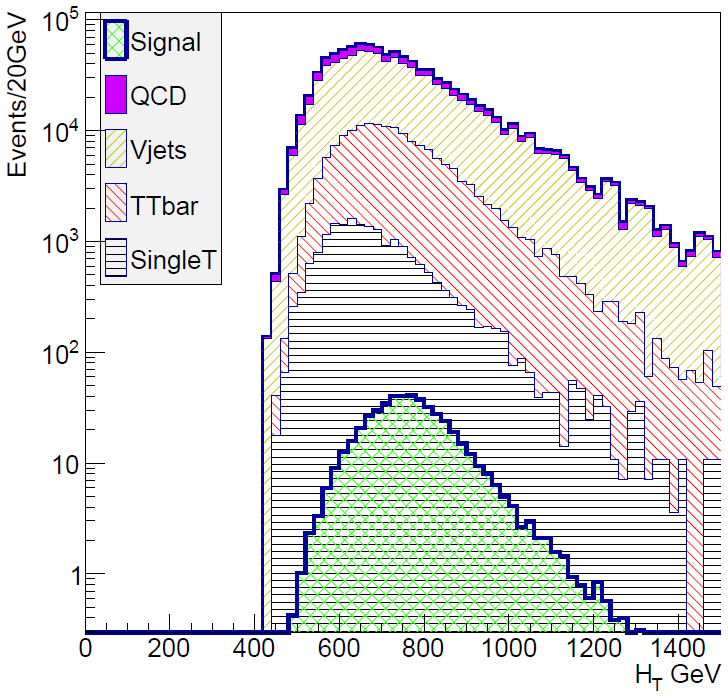
\includegraphics[width=0.8\textwidth]{figs/Ana/HT.png}
    \caption{Distribution of the $H_{T}$ variable for data and the sum of the MC samples normalized to luminosity. The signal sample (M=700 \GeVcc) is over-imposed on top of the stack of the MC samples. The gray band represents the statistical uncertainties from the sum of the MC background. Reasonable agreement is observed, with the multijet process as the dominant process at this stage. Normalization of samples done to luminosity on data.}
    \label{fig:HT}
  \end{center}
\end{figure}

The final cut of the basic selection concerns the request of a minimum number of b-tagged jets. The CSV algorithm (described in section~\ref{sec:bid}) was used to identify jets coming from a b quark. In the following, b-tagged jets are defined as jets that were b-tagged by the CSV algorithm and b-jets as jets truly coming from a b-quark (from matrix element). The medium working point was chosen as it allows to have a high efficiency on b-jet identification (70\%) with a low fake rate from c (20\%) and light quarks (1\%) and it allows to keep a high efficiency on signal~\cite{Chatrchyan:2012jua, CMS:2013vea}. In the full hadronic final state, the \Tp decays in three b-quarks, a \bbbar system coming from the Higgs and an additional b quark from the t-quark, and two light jets from the W boson produced by the top. Accordingly, signal events are expected to have at least 3 b-tagged jets, while \ttbar~and QCD events should have 2.

In principle several working points can be used to establish the b-tagged jets content of events. For example, events can be required to have at least 3 b-tagged jets one with tight working point and two with medium working points. All possible combinations have been studied from the three available working points (loose (CSVL), medium (CSVM) and tight (CSVT)) to require at least 3 CSV b-tagged jets in order to establish which combination gave the best $S/B$ while keeping the most of signal events. For the study, we have used as signal the $M=700$ \GeVcc signal sample and as backgrounds the \ttbar, QCD\_HT-500To1000 and QCD\_HT-1000ToInf MC samples. The study was performed applying the basic selection, after \HT~cut. The results of the study are contained in table~\ref{tab:BCutStudy}. From this table, it can be seen that the most efficient cuts to discriminate signal from backgrounds and to keep signal are to require at least 3 CSVM b-tagged jets or to require at least 2 CSVM and 1 CSVT b-tagged jets. For simplicity of the reconstruction procedure and the background estimation, at least 3 CSVM b-tagged jets are required. At this stage it is extremely important to keep enough signal, because the next step of the analysis involves the reconstruction of the \Tp.

\begin{table}[htbH]
\begin{center}
\resizebox{\textwidth}{!}{
\begin{tabular}{| c || c | c | c | c | c | c |}
\hline 
\textit{At least} & $\epsilon(S)$ [\%] & $\epsilon(t\bar{t})$ [\%] & $\epsilon(\text{QCD\_HT-500To1000})$ [\%] & $\epsilon(\text{QCD\_HT-1000ToInf})$ [\%] & $\frac{S}{B}\times 10^{3}$ & $\frac{S}{S+B}\times 10^{2}$ \\
\hline
3 CSVL                       & $65 \pm 0.4$  & $38 \pm 0.04$  & $6 \pm 0.02$    & $7 \pm 0.02$     & $0.4 \pm 0.005$  & $24.8 \pm 0.3$ \\
3 CSVM                       & $31 \pm 0.4$  & $8 \pm 0.02$   & $1 \pm 0.01$    & $0.6 \pm 0.01$   & $1.8 \pm 0.05$   & $38.2 \pm 0.8$ \\
1 CSVL and 2 CSVM            & $55 \pm 0.4$  & $27 \pm 0.03$  & $2 \pm 0.01$    & $2 \pm 0.01$     & $0.8 \pm 0.01$   & $33.7 \pm 0.5$ \\
2 CSVL and 1 CSVM            & $64 \pm 0.4$  & $37 \pm 0.04$  & $5 \pm 0.02$    & $5 \pm 0.02$     & $0.5 \pm 0.007$  & $28.3 \pm 0.3$  \\
2 CSVM and 1 CSVT            & $29 \pm 0.4$  & $8 \pm 0.02$   & $0.5 \pm 0.006$ & $0.5 \pm 0.006$  & $1.9 \pm 0.05$   & $38.4 \pm 0.8$  \\
1 CSVM and 2 CSVT            & $22 \pm 0.4$  & $5 \pm 0.02$   & $0.3 \pm 0.005$ & $0.3 \pm 0.003$  & $2.2 \pm 0.07$   & $35.8 \pm 0.9$  \\
3 CSVT                       & $9 \pm 0.2$   & $1 \pm 0.01$   & $0.1 \pm 0.003$ & $0.09 \pm 0.002$ & $3.1 \pm 0.2$    & $27.3 \pm 1.1$  \\
1 CSVL and 2 CSVT            & $33 \pm 0.4$  & $13 \pm 0.03$  & $0.9 \pm 0.01$  & $0.8 \pm 0.007$  & $1.1 \pm 0.03$   & $31.5 \pm 0.6$  \\
2 CSVL and 1 CSVT            & $57 \pm 0.4$  & $30 \pm 0.03$  & $3 \pm 0.02$    & $3 \pm 0.01$     & $0.7 \pm 0.01$   & $31.5 \pm 0.4$  \\
1 CSVL and 1 CSVM and 1 CSVT &  $51 \pm 0.4$ &  $24 \pm 0.03$ & $2 \pm 0.01$    & $2 \pm 0.01$     & $0.9 \pm 0.02$   & $30.8 \pm 0.4$  \\
\hline

\hline
\end{tabular}
}
\caption{Comparative study of different possible combinations to require at least 3 b-tagged jets with CSVL, CSVM and CSVT working points. Efficiencies of cuts over signal and principal MC background samples are presented, as well as $\frac{S}{B}$ and $\frac{S}{S+B}$. We chose the cut giving highest $\frac{S}{S+B}$, at least 3CSVM. High values of $\frac{S}{S+B}$ point to a good discrimination while keeping the signal efficiency high.\label{tab:BCutStudy}}
\end{center}
\end{table}

Additionally, the 2D plots relating the number of b-tagged jets in the three working points for signal after requiring $j^{1}>150$ GeV/c and $H_{T}>550$ GeV/c can be found in figure~\ref{fig:WPcorr}.

\begin{figure}[!Hhtbp]
  \begin{center}
    \includegraphics[width=0.65\textwidth, height=0.3\textheight]{figs/Ana/CSVMCSVT.png}
    \includegraphics[width=0.65\textwidth, height=0.3\textheight]{figs/Ana/CSVTCSVL.png}
    \includegraphics[width=0.65\textwidth, height=0.3\textheight]{figs/Ana/CSVMCSVL.png}
    \caption{Correlation plots between different b-tagging working points for signal MC sample (M=700 \GeVcc) with selection up to $H_{T}>550$ GeV/c. Numbers in each bin correspond to its Number of entries. CSVM with CSVT [top], CSVT with CSVL [medium] and CSVM with CSVL [bottom]. Numbers in each bin correspond to the number of entries in the bin.}
    \label{fig:WPcorr}
  \end{center}
\end{figure}

As described in section~\ref{sec:bid} the b-tagging is performed using a procedure where several jet variables are taken into account. It strongly depends on the ability to find displaced vertices, reason why it has been restricted to jets in $|\eta|<=2.4$. As MC conditions are ideal in comparison with real data, the b-tagging performance are different in data and in MC. Thus, a correction must be applied to MC to mimic b-tagging response on data. In general, the CSV algorithm is slightly more efficient for b-tagging b-jets in MC than in data, and b-tag more light jets as b-jets in data than in MC. To match MC to data a scale factor has been derived by the collaboration. It is defined for each jet depending on its flavor (b and c or light), \pt and $\eta$. In equation~\ref{eq:Sfs}~\cite{CMS:2013vea}, the parametrization of the scale factors for CSVM working point can be found. The functions are defined as $SF^{flavor}_{\eta}(p_{T})$.

\begin{eqnarray}
  \label{eq:Sfs}
  SF^{b\; or\; c}_{|\eta|\le 2.4}(x) & = & 0.938887 + 0.00017124x - 2.76366 \times 10^{-7}x^{2} \nonumber \\
  SF^{light}_{|\eta|\le 0.8}(x) & = & 1.07541 + 0.00231827x - 4.74249 \times 10^{-6}x^{2}  \nonumber \\
  &  & +2.70862 \times 10^{-9}x^{3} \nonumber \\
  SF^{light}_{0.8 < |\eta|\le 1.6}(x) & = & 1.05613 + 0.00114031x - 2.56066 \times 10^{-6}x^{2} \nonumber \\
  &  & + 1.67792 \times 10^{-9}x^{3} \nonumber \\
  SF^{light}_{1.6 < |\eta|\le 2.4}(x) & = & 1.05625 + 0.000487231x - 2.22792 \times 10^{-6}x^{2} \nonumber \\
  &  & + 1.70262 \times 10^{-9}x^{3}
\end{eqnarray}

In order to apply the b-tagging scale factors to MC samples, a method approved by the collaboration was used. The chosen method allows to calculate a weight per events in terms of its jet flavor content. The weight definition can be found in equation~\ref{eq:SFW}, 

\begin{equation}
  \label{eq:SFW}
  w=\frac{P(\text{DATA})}{P(\text{MC})}
\end{equation}where

\begin{eqnarray}
  \label{eq:DataMCSFP}
  P(\text{MC}) & = & \prod_{i=\text{tagged}} \varepsilon_i \prod_{j=\text{not tagged}} (1-\varepsilon_j) \\
  P(\text{DATA}) & = & \prod_{i=\text{tagged}} \text{SF}_i \varepsilon_i \prod_{j=\text{not tagged}} (1-\text{SF}_j \varepsilon_j)
\end{eqnarray}the products are defined over all jets in the event. $\varepsilon$ represents the b-tagging efficiency. Efficiencies were calculated for each MC sample as function of flavor, \pt and $\eta$. In figure~\ref{fig:ttbarBEff} the CSVM b-tagging efficiencies for b, c and light jet flavors for \ttbar MC sample can be found. Also, the calculated weights for each MC sample are shown in figure~\ref{fig:SFweight}. 

%\begin{figure}[!Hhtbp]
%  \begin{center}
%    \includegraphics[width=0.8\textwidth, height=0.33\textheight]{figs/Ana/Signal_beff.png}
%    \includegraphics[width=0.8\textwidth, height=0.33\textheight]{figs/Ana/Signal_ceff.png}
%    \includegraphics[width=0.8\textwidth, height=0.33\textheight]{figs/Ana/Signal_leff.png}
%    \caption{CSVM b-tagging efficiency for b-jets [left], c-jets [center] and light jets [right] as function of \pt and $\eta$ for signal M=700 \GeVcc.}
%    \label{fig:SignalBEff}
%  \end{center}
%\end{figure}

\begin{figure}[!Hhtbp]
  \begin{center}
    \includegraphics[width=0.8\textwidth, height=0.3\textheight]{figs/Ana/ttbar_beff.png}
    \includegraphics[width=0.8\textwidth, height=0.3\textheight]{figs/Ana/ttbar_ceff.png}
    \includegraphics[width=0.8\textwidth, height=0.3\textheight]{figs/Ana/ttbar_leff.png}
    \caption{CSVM b-tagging efficiency for b-jets [left], c-jets [center] and light jets [right] as function of \pt and $\eta$ for \ttbar.}
    \label{fig:ttbarBEff}
  \end{center}
\end{figure}

%\begin{figure}[!Hhtbp]
%  \begin{center}
%    \includegraphics[width=0.8\textwidth, height=0.33\textheight]{figs/Ana/QCDHT500_beff.png}
%    \includegraphics[width=0.8\textwidth, height=0.33\textheight]{figs/Ana/QCDHT500_ceff.png}
%    \includegraphics[width=0.8\textwidth, height=0.33\textheight]{figs/Ana/QCDHT500_leff.png}
%    \caption{CSVM b-tagging efficiency for b-jets [left], c-jets [center] and light jets [right] as function of \pt and $\eta$ for QCD\_HT-500To1000.}
%    \label{fig:QCDBEff}
%  \end{center}
%\end{figure}

\begin{figure}[!Hhtbp]
  \begin{center}
    \includegraphics[width=0.8\textwidth]{figs/Ana/SF_weight.png}
    \caption{Distribution of the weights from b-tagging scale factors for all MC samples.}
    \label{fig:SFweight}
  \end{center}
\end{figure}

Efficiencies were calculated using the following formula:

\begin{equation}
  \label{eq:btaggingeff}
  \varepsilon_f(i,j) = \frac{N_f^\text{b-tagged}(i,j)}{N_f^\text{Total}(i,j)}
\end{equation} where $ N_f^\text{Total}(i,j) $ and $ N_f^\text{b-tagged}(i,j) $ are the total number and the number of b-tagged jets, respectively, of flavor $ f $ in the $ (p_\text{T},\eta) $ bin $ (i,j) $. The determination of the jet flavor is done via the matching of jets to quarks from parton level simulation. The matching is not always successful and some jets can have no parton matched, i.e. no associated flavor. These jets, as well as jets coming from gluons, were included in the light flavor category.

Finally, data were compared to the MC predictions in figure~\ref{fig:Nb} in the number of CSVM b-tagged jets. The different data/MC comparisons presented are used for illustration and to check that pileup and b-tagging corrections in MC are correctly applied. For the final analysis results only signal MC samples are used, as backgrounds were estimated directly from the data.

\begin{figure}[!Hhtbp]
  \begin{center}
    \includegraphics[width=0.8\textwidth]{figs/Ana/NCSVM.png}
    \caption{B-tagged CSVM jet multiplicity for data and MC samples before requiring at least 3 CSVM b-tagged jets. The sum of MC is normalized to the integrated luminosity in the data.}
    \label{fig:Nb}
  \end{center}
\end{figure}
%\begin{TOINCLUDE}Plots of pt and eta of six leading jets, number of vertices, HT and number of CSVM b-tagged jets\end{TOINCLUDE}

\subsection{\Tp~reconstruction with a $\chi^{2}$ sorting algorithm}
\label{sec:chi2}

A crucial step to reconstruct the \Tp~mass is to correctly identify the five jets coming from its decay. Events passing the basic selection have at least 6 jets, but jet multiplicity can be much greater. Additionally, there are several possible combinations between jets to reconstruct the Higgs boson and top quark form the \Tp~decay. In consequence, the process of identification of jets coming from the \Tp~is not trivial. 

A $\chi^{2}$ sorting algorithm has been used to identify the \Tp~decay products and to reconstruct the Higgs and top. This technique relies in the definition of a $\chi^{2}$ variable for each jets combination in an event. The combination that minimizes this variable gives the best fit of the objects under reconstruction. An example of this method can be found in~\cite{Brochet:1956723}. 

The $\chi^{2}$ variable is defined in equation~\ref{eq:chi2def}. The values used as inputs were: $M_{H}=125$~\GeVcc, $M_{W}=84.06$~\GeVcc, $M_{t}=175.16$~\GeVcc, $\sigma_{H}=12.4$~\GeVcc, and $\sigma_{W}=10.12$~\GeVcc and $\sigma_{t}=17.35$~\GeVcc. These values were taken from \cite{Brochet:1956723,Chatrchyan:2013zna}, where similar studies of a $\chi^{2}$ reconstruction of these particles in full hadronic final state were performed. For the Higgs reconstruction only CSVM b-tagged jets are considered. For the W reconstruction all jets with a \ptg{30} were considered, while for the top reconstruction one b-tagged jet and the pair of jets used for the W. %B-tagging status of jets used for the W was not used.

\begin{equation}
\chi^{2}=\frac{(M_{H}-M_{bb})^{2}}{\sigma_{H}^{2}}+\frac{(M_{W}-M_{jj})^{2}}{\sigma_{W}^{2}}+\frac{(M_{t}-M_{bjj})^{2}}{\sigma_{t}^{2}}
\label{eq:chi2def}
\end{equation}

The efficiency of the reconstruction of each particle (Higgs, \W, top and \Tp) can be evaluated using signal MC samples shown in table~\ref{tab:MCsig}. Two efficiencies are defined, the exclusive efficiency as the ratio between the number of events where the particle was well reconstructed and the number of events where all jets where correctly matched to a parton, and the inclusive efficiency where the ratio is done with respect to the total number of events. Both efficiencies were evaluated after basic selection. The efficiency values are shown in figure~\ref{fig:RecEff}. We found an exclusive efficiency of around 70\% for the \Tp~independently of its mass.

\begin{figure}[!Hhtbp]
  \begin{center}
    \includegraphics[width=0.46\textwidth]{figs/Ana/Exclusive_Efficiency_V8.png}
    \includegraphics[width=0.46\textwidth]{figs/Ana/Inclusive_Efficiency_V8.png}
    \caption{Efficiency of reconstruction by the $\chi^{2}$ algorithm of the Higgs, \W, top and \Tp~taking into account only events where jets could be matched to partons [left] and to total number of events [right]}
    \label{fig:RecEff}
  \end{center}
\end{figure}

In figure~\ref{fig:WHt} the W, Higgs and top masses reconstructed by the $\chi^{2}$ sorting algorithm are shown. Additionally, in figure~\ref{fig:RecT} the reconstructed \Tp~mass for all used signal MC samples is shown. Finally, in table~\ref{tab:SignalWidths} are presented the results from fitting with a gaussian all mass points after full selection (the rest of the selection is presented in section~\ref{sec:finalsel}). The found widths for the \Tp~mass vary between 30 to 50 \GeVcc, about 6\% of \Tp~mass. This fit is used to calculate the expected yields for the signal for the calculation of limits (see sections~\ref{sec:sys} and~\ref{sec:res}).

\begin{figure}[!Hhtbp]
  \begin{center}
    \includegraphics[width=0.32\textwidth]{figs/Ana/TopMass_S700.png}
    \includegraphics[width=0.32\textwidth]{figs/Ana/WMass_S700.png}
    \includegraphics[width=0.32\textwidth]{figs/Ana/HiggsMass_S700.png}
    \caption{Reconstructed top, \W~and \Hb~for the \Tp~mass point of 700 \GeVcc}
    \label{fig:WHt}
  \end{center}
\end{figure}

\begin{figure}[!Hhtbp]
  \begin{center}
    \includegraphics[width=0.45\textwidth]{figs/Ana/HundresdsMassChi2Tp.png}
    \includegraphics[width=0.45\textwidth]{figs/Ana/FiftiesMassChi2Tp.png}
    \caption{Reconstructed \Tp~mass for all mass points from the $\chi^{2}$ sorting algorithm after basic selection. Each mass point is normalized to luminosity in the data and its corresponding cross section. }
    \label{fig:RecT}
  \end{center}
\end{figure}

\begin{table*}[htbH]
\begin{center}
\begin{tabular}{|c|c|c|c|c|}
\hline 
\multicolumn{2}{|c}{Generated} & \multicolumn{3}{|c|}{Reconstructed} \\
Mass (GeV/$c^{2}$) & Width (GeV/$c^{2}$) & Mass (GeV/$c^{2}$) & Width (GeV/$c^{2}$) & $\chi^{2} /$ndf\\
\hline
600 & 0.62 &$604.60\pm14.18$ & $32.44\pm10.37$ & 4.99/4\\
650 & 0.80 &$644.56\pm12.64$ & $35.53\pm9.54$ & 8.03/4\\
700 & 1.02 &$691.79\pm13.65$ & $41.16\pm9.75$ & 10.80/7\\
750 & 1.27 &$736.26\pm15.53$ & $45.38\pm11.46$ & 10.24/7\\
800 & 1.56 &$782.97\pm18.12$ & $49.35\pm13.49$ & 23.67/7\\
850 & 1.89 &$832.49\pm17.92$ & $47.39\pm13.28$ & 15.71/7\\
900 & 2.26 &$881.38\pm19.13$ & $45.58\pm14.24$ & 11.01/7\\
950 & 2.67 &$929.02\pm25.02$ & $51.54\pm18.96$ & 14.54/7\\
1000 & 3.13 &$970.36\pm32.18$ & $53.34\pm25.14$ & 11.51/7\\
\hline
\end{tabular}
\caption{Reconstructed mass and width for \Tp~candidate after full analysis selection from a gaussian fit for each signal mass generated. \label{tab:SignalWidths}}
\end{center}
\end{table*}

The $\chi^{2}$ distribution is plotted in figure~\ref{fig:chi2}. Signal events have preferentially a $\chi^{2}<50$, while multijet and \ttbar backgrounds have much longer tails at higher $\chi^{2}$ values.

\begin{figure}[!Hhtbp]
  \begin{center}
    \includegraphics[width=0.8\textwidth]{figs/Ana/chi2Nm1.png}
    \caption{Distribution of the $\chi^{2}$ variable for data and MC samples. The signal sample used has a \Tp~mass of 700 \GeVcc. Backgrounds present higher values than the signal. The sum of MC is normalized to the integrated luminosity in the data.}
    \label{fig:chi2}
  \end{center}
\end{figure}
%\begin{TOINCLUDE}Table with inclusive and exclusive reconstruction efficiency. Plots of mass of reconstructed T, W, H and top right after reconstruction for all mass points. Table with gaussian fit results.\end{TOINCLUDE}

\subsection{Selection based on reconstructed objects}
\label{sec:finalsel}

After the reconstruction procedure, a final step in the selection is performed based on the properties of the reconstructed resonances. This last set of cuts has been optimized to obtain the highest discrimination between signal and backgrounds. The discrimination of the selection has been evaluated from the estimator $S/B$, where the signal MC sample with $M(T)=700$ \GeVcc, and the \ttbar and QCD\_HT-500To1000 samples for the backgrounds have been used. These two background samples have the highest contribution to the invariant mass of five jets between 600 and 1000 \GeVcc. For optimization purposes, the selection has been adjusted to keep at least 10 signal events after the full selection.

The main limitation for the optimization of the selection is the lack of statistics in the multijet MC sample. It is to be kept in mind that the plots with data MC comparison are shown for illustration only, since the limit setting and final results were produced with an estimation of backgrounds derived form the data.

The first variable considered for the selection is the $\chi^{2}$ distribution. As seen in figure~\ref{fig:chi2}, the signal tends to have smaller values of $\chi^{2}$ than the backgrounds. In figure~\ref{fig:chi2cut}, a scan of the efficiency of cutting on the $\chi^{2}$ for the values displayed in the x-axis can be seen. These efficiencies were evaluated for the signal ($M(T)=700$ \GeVcc), \ttbar and QCD\_HT-500To1000 MC samples. In addition, the ratio of the efficiency of signal over the efficiency of the cut on \ttbar and QCD samples are shown. These ratios are directly proportional to $S/B$. In agreement with the increase of $S/B$ as measure of the cut value, a cut on $\chi^{2}<8$ has been chosen. One additional feature of this cut, that will be seen in section~\ref{sec:bkg}, is that it ensures the agreement of the control sample with the signal sample for the background estimation. 

\begin{figure}[!Hhtbp]
  \begin{center}
    \includegraphics[width=0.8\textwidth]{figs/Ana/chi2_SoB.png}
    \caption{Efficiency of selection criterion $\chi^{2}<x$, with $x$ the cut value, as function of the cut value for \Tp~with $M=700$ \GeVcc, \ttbar and QCD\_HT-500To1000 MC samples. Ratios between efficiency for signal and each background are also displayed.}
    \label{fig:chi2cut}
  \end{center}
\end{figure}

After cutting in $\chi^{2}$, events were required to have the two b-quarks used to reconstruct the Higgs boson at a distance $\Delta R(bb)<1.2$. As in signal events the Higgs boson is produced by the massive \Tp, it is expected to be produced with a high \pt. Therefore, the decay products from the Higgs, the \bbbar~system, are expected to be close in the $\eta-\phi$ plane. In figure~\ref{fig:DRbb} the comparison between data and MC on $\Delta R(bb)$ is shown before cutting on this variable. In the same figure the efficiency of cutting on different values for each MC sample used in the optimization is shown, altogether with the efficiency ratios. %It is also shown an equivalent cut efficiency study as for $\chi^{2}$ variable. 

\begin{figure}[!Hhtbp]
  \begin{center}
    \includegraphics[width=0.45\textwidth]{figs/Ana/DRbbNm1.png}
    \includegraphics[width=0.45\textwidth]{figs/Ana/DRbb_SoB.png}
    \caption{$\Delta R$ of the 2 b-tagged jets used to reconstruct the Higgs candidate after $\chi^{2}$ cut. The signal which is simply overlaid prefers low $\Delta R$ while backgrounds have larger distribution at higher value. The gray band represents the statistical uncertainties from the sum of the MC background. Normalization was done to luminosity on the data [right]. Efficiency of selection criterion $\Delta R(bb)<x$, with $x$ the cut value, as function of cut value for $M=700$ \GeVcc signal sample, \ttbar and QCD\_HT-500To1000 MC samples and ratios between efficiency for signal and each background [left].}
    \label{fig:DRbb}
  \end{center}
\end{figure}

Events were then required to have a reconstructed \W and \Hb with $1.6<\Delta R (W_{cand} H_{cand})<4.0$. This variable presents a peak for signal at 2.8, as shown in figure~\ref{fig:DRWH}. Backgrounds also have a peak around 3, but have larger tails than the signal. The cut has been chosen to keep events inside a window of 1.2 around the peak. In the same figure, the cut efficiency plot for this variable for different window values is also shown.

\begin{figure}[!Hhtbp]
  \begin{center}
    \includegraphics[width=0.45\textwidth]{figs/Ana/DRWHNm1.png}
    \includegraphics[width=0.45\textwidth]{figs/Ana/DRWH_SoB.png}
    \caption{Distribution for $\Delta R (W_{cand} H_{cand})$ for data and the sum of Monte Carlo samples [left]. Efficiency of selection criterion $|\Delta R(W_{cand} H_{cand})-2.8|<x$, with $x$ the cut value, as function of cut value for the $M=700$ \GeVcc signal sample, \ttbar and QCD\_HT-500To1000 MC samples and ratios between efficiency for signal and each background [right]. All others selection criteria are applied up to this one.}
    \label{fig:DRWH}
  \end{center}
\end{figure}

One important difference between signal and backgrounds is that in signal events there is a \bbbar~system coming from the decay of a Higgs boson. Thus, a resonance peak is expected to appear for the \bbbar system for signal events, while it is not the case for backgrounds. In consequence, events were required to have a Higgs candidate mass between 105 and 145 \GeVcc. The efficiency plot of cutting on events outside a window around 125 \GeVcc in the Higgs candidate mass is shown in figure~\ref{fig:HiggsMassDMC}. In the same figure the Higgs candidate mass is shown, before cutting on it, for the data and MC samples.

\begin{figure}[!Hhtbp]
  \begin{center}
    \includegraphics[width=0.45\textwidth]{figs/Ana/HMNm1.png}
    \includegraphics[width=0.45\textwidth]{figs/Ana/HM_SoB.png}
    \caption{Distribution for $M(H_{cand})$ for data and the sum of Monte Carlo samples [left]. Efficiency of selection criterion $|M(H_{cand})-125|<x$, with $x$ the cut value, as function of cut value for the $M=700$ \GeVcc signal sample, \ttbar and QCD\_HT-500To1000 MC samples and ratios between efficiency for signal and each background [right]. All others selection criteria are applied up to this one.}
    \label{fig:HiggsMassDMC}
  \end{center}
\end{figure}

Due to the presence of a real top in \ttbar~events, this background is able to mimic the signal properties more likely than QCD. To understand how the \ttbar system is mimicking a Higgs boson, the MC truth information of the jets chosen by the $\chi^{2}$ sorting algorithm as coming from the Higgs have been. In figure~\ref{fig:RecohiggsMCTruth} the Higgs reconstruction cases can be seen. %, coded as follows:

%\begin{itemize}
%\item Bin 0: Higgs candidate reconstructed from two b-quarks coming each one from a top quark.
%\item Bin 1: Higgs candidate reconstructed from Higgs \bbbar system.
%\item Bin 2: Higgs candidate reconstructed from one quark from the Higgs and one b-quark from a top.
%\item Bin 3: Higgs candidate reconstructed from one quark from the Higgs and one quark from a W.
%\item Bin 4: Higgs candidate reconstructed from one b-quark from the top and one quark from a W.
%\item Bin 5: Higgs candidate reconstructed from two quarks coming from W bosons.
%\item Bin 6: Higgs candidate reconstructed from one jet from the Higgs and one additional quark (not from Higgs, W nor top).
%\item Bin 7: Higgs candidate reconstructed from one b-quark from a top and one additional quark (not from Higgs, W nor top).
%\item Bin 8: Higgs candidate reconstructed from one jet from a W and one additional quark (not from Higgs, W nor top).
%\item Bin 9: Higgs candidate reconstructed from two additional quarks (not from Higgs, W nor top).
%\end{itemize}

\begin{figure}[!Hhtbp]
  \begin{center}
    \includegraphics[width=0.45\textwidth]{figs/Ana/HiggsRecoMCTruth_S700.png}
    \includegraphics[width=0.45\textwidth]{figs/Ana/HiggsRecoMCTruth_TTJets.png}
    \captionsetup{singlelinecheck=off}
    \caption[list=off]{Higgs candidate reconstruction MC truth for signal (M=700 \GeVcc) [left] and \ttbar [right] MC samples. In signal the Higgs is reconstructed preferentially from two jets coming from the Higgs (bin 1) while for \ttbar~the Higgs candidate is reconstructed preferentially from a b-quark from a top and a quark from a \W boson (bin 4). The bins are defined as follows:\\
\scalebox{0.8}{%
\vbox{%
\begin{description}
\item[Bin 0:] Higgs candidate reconstructed from two b-quarks coming each one from a top quark.
\item[Bin 1:] Higgs candidate reconstructed from Higgs \bbbar~system.
\item[Bin 2:] Higgs candidate reconstructed from one quark from the Higgs and one b-quark from a top.
\item[Bin 3:] Higgs candidate reconstructed from one quark from the Higgs and one quark from a \W.
\item[Bin 4:] Higgs candidate reconstructed from one b-quark from the top and one quark from a \W.
\item[Bin 5:] Higgs candidate reconstructed from two quarks coming from \W~bosons.
\item[Bin 6:] Higgs candidate reconstructed from one jet from the Higgs and one additional quark (not from Higgs, \W~nor top).
\item[Bin 7:] Higgs candidate reconstructed from one b-quark from a top and one additional quark (not from Higgs, \W~nor top).
\item[Bin 8:] Higgs candidate reconstructed from one jet from a \W~and one additional quark (not from Higgs, \W~nor top).
\item[Bin 9:] Higgs candidate reconstructed from two additional quarks (not from Higgs, \W nor top).
\end{description}}}}
    \label{fig:RecohiggsMCTruth}
  \end{center}
\end{figure}

In this figure one can see that the Higgs candidate is preferentially reconstructed in \ttbar~events from a b-quark coming from a top and one quark coming from a \W~boson. As one top is also reconstructed, this means that the Higgs is being reconstructed from the second top. Thus, to identify \ttbar~events the b-tagged jets used for the Higgs and one additional jet not used by the $\chi^{2}$ algorithm can be used to reconstruct the second top. As this extra jet is coming from a top is expected to be have a significant amount of \pt, then the second top is reconstructed from the two Higgs jets and the leading jet not used by the $\chi^{2}$ algorithm. A second \W~is also defined from the sub-leading Higgs jet and leading jet not used by the $\chi^{2}$ algorithm. This definition follows the expectation that the jet with highest \pt~from top decay is the b-quark coming directly from it. The distribution for the second top mass can be seen in figure~\ref{fig:2ndTM} for data and MC samples. The top mass peak is clearly reproduced by \ttbar~events.

\begin{figure}[!Hhtbp]
  \begin{center}
    \includegraphics[width=0.45\textwidth]{figs/Ana/M2ndTopNm1.png}
    \caption{Second top mass distribution for data and the sum of the Monte Carlo samples. Selection criteria are applied up to Higgs mass cut. The second top is reconstructed from the two Higgs jets and the leading jet not used by the $\chi^{2}$ algorithm. The normalization was done to luminosity on the data.}
    \label{fig:2ndTM}
  \end{center}
\end{figure}

A variable with the second top and second \W~boson to discriminate signal from background (mainly \ttbar) has bee built. To increase the separation between backgrounds and signal not only the second top mass is taken, but added to the second \W~boson mass and this sum divided by the Higgs mass. The distribution for this variables is shown in figure~\ref{fig:m2thp} for data and the sum of MC samples. Events with $(M(top^{2nd})+M(W^{2nd}))/M(H)>6.8$ were selected.

\begin{figure}[!Hhtbp]
  \begin{center}
    \includegraphics[width=0.45\textwidth]{figs/Ana/M2HPNm1.png}
    \includegraphics[width=0.45\textwidth]{figs/Ana/M2HP_SoB.png}
    \caption{Distribution of $(M(top^{2nd})+M(W^{2nd}))/M(H)$ for data and the sum of the Monte Carlo samples. Selection criteria are applied up to Higgs mass cut. The low statistics in the multijet (QCD) MC sample is visible at this stage. The gray band represents the statistical uncertainties from the sum of the MC background and it is dominated by QCD samples [left]. Efficiency of selection criterion $(M(top^{2nd})+M(W^{2nd}))/M(H)>x$, with $x$ the cut value, as function of cut value for $M=700$ \GeVcc signal sample, \ttbar and QCD\_HT-500To1000 MC samples and ratios between efficiency for signal and each background [right].}
    \label{fig:m2thp}
  \end{center}
\end{figure}

The selection continues taking advantage of the angular relation between the \Tp~and the quark produced in association with it for signal events. They are produced preferentially with high $\Delta R$ while for backgrounds the two objects have lower $\Delta R$. The leading jet not used by the reconstruction procedure is defined as the jet produced in association to the \Tp. This jet will be referred as the 6th jet, $j^{6}$. The distribution of $\Delta R (T j^{6th})$ can be found in figure~\ref{fig:jet6} for data and MC samples along with the efficiency plot of cutting on $\Delta R (T j^{6})$ for $M=700$ \GeVcc signal sample, \ttbar and QCD\_HT-500To1000 MC samples. At this stage the statistics in QCD MC samples begin to be very low. Events that have $\Delta R (T j^{6})>4.8$ were selected. 

\begin{figure}[!Hhtbp]
  \begin{center}
    \includegraphics[width=0.45\textwidth]{figs/Ana/DRTp6JNm1.png}
    \includegraphics[width=0.45\textwidth]{figs/Ana/DRTp6thJ_SoB.png}
    \caption{Distributions for $\Delta R (T j^{6th})$  for data and the sum of Monte Carlo samples. All others criteria are applied up to this one. The low statistics in the multijet (QCD) MC sample is visible at this stage. The gray band represents the statistical uncertainties from the sum of the MC background and it is dominated by QCD samples [left]. Efficiency of selection criterion $\Delta R (T j^{6th})>x$, with $x$ the cut value, as function of cut value for $M=700$ \GeVcc signal sample, \ttbar and QCD\_HT-500To1000 MC samples and ratios between efficiency for signal and each background [right].}
    \label{fig:jet6}
  \end{center}
\end{figure}

For the last criterion the Relative $H_{T}$ variable is defined as the sum of the \pt~of the Higgs candidate plus the \pt~of the top candidate divided by $H_{T}$ of the event. This variable is related to the proportion of \HT~of the event coming from the Higgs boson and top candidates \pt. As for signal events the top and Higgs boson candidates are coming from a highly massive object, that is decaying into a top and a Higgs, signal events have a relative $H_{T}$ closer to 1 than backgrounds events. The relative $H_{T}$ distribution is shown in figure~\ref{fig:RelHtMass} for data and the sum of MC samples before cutting on it, with the rest of the selection applied. At this stage the QCD MC samples have very low statistics. In the same figure can be found the efficiency plot of the cut. We keep events that have a Relative $H_{T}>0.67$. 

\begin{figure}[!Hhtbp]
  \begin{center}
    \includegraphics[width=0.45\textwidth]{figs/Ana/RelHTNm1.png}
    \includegraphics[width=0.45\textwidth]{figs/Ana/RelHT_SoB.png}
    \caption{Distribution of Relative $H_{T}$ for data and the sum of the Monte Carlo samples. All others criteria are applied up to this one. At this stage multijet (QCD) MC sample have very low statistics. The gray band represents the statistical uncertainties from the sum of the MC background and it is dominated by QCD samples [left]. Efficiency of selection criterion Relative $H_{T}>x$, with $x$ the cut value, as function of cut value for $M=700$ \GeVcc signal sample, \ttbar and QCD\_HT-500To1000 MC samples and ratios between efficiency for signal and each background [right]. }
    \label{fig:RelHtMass}
  \end{center}
\end{figure}

To check the evolution of the selection, in table~\ref{tab:Estimators} is shown the $S/B$ after each cut after the reconstruction of resonances with the $\chi^{2}$ algorithm. In the table an increase of the estimator is visible at each step, which means that with each cut the discrimination between signal and background increases. As a reminder, $M=700$ \GeVcc signal, \ttbar and QCD\_HT-500To1000 MC samples were used for this calculation. %As QCD statistics decrease rapidly, and at some point they are very low, we calculate the estimator with respect to \ttbar and QCD samples separately.

\begin{table}[htbH]
\begin{center}
%\resizebox{\textwidth}{!}{
\begin{tabular}{|c|c|c|}
\hline 
Cut & $S/B$ & $S/\sqrt{S+B}$ \\
\hline
$\chi^{2}<8$ & $3.4\ex{-2} \pm 2.85\ex{-3}$  & $ 0.96 \pm 0.05$  \\
$\Delta R(bb)<1.2$ & $4.76\ex{-2} \pm 4.52\ex{-3}$ & $1.10 \pm 0.07$  \\
$1.6<\Delta R (W_{cand} H_{cand})<4.0$ & $4.82\ex{-2} \pm 4.59\ex{-3}$  & $1.10 \pm 0.07$  \\
$105$ \GeVcc $< M(H_{cand}) < 145$ \GeVcc & $6.38\ex{-2} \pm 6.81\ex{-3}$  & $1.21 \pm 0.08$  \\
$(M(top^{2nd})+M(W^{2nd}))/M(H_{cand})>6.8$ & $0.15 \pm 0.03$  & $1.45 \pm 0.17$  \\
$\Delta R (T j^{6th})>4.8$ & $0.42 \pm 0.19$  & $1.66 \pm 0.32$  \\
Relative $H_{T}>0.67$ & $1.16 \pm 0.17$  & $2.13 \pm 0.17$  \\
\hline
\end{tabular}
\caption{$S/B$ and $S/\sqrt{S+B}$ from MC samples for each step of the selection after reconstruction of resonances with the $\chi^{2}$ sorting algorithm. Only $M=700$ \GeVcc signal, \ttbar and QCD\_HT-500To1000 MC samples were used. \label{tab:Estimators}}
%}
\end{center}
\end{table}
%\begin{TOINCLUDE}$N-1$ plots for object selection variables. Table with $S/B$ and $S/\sqrt{S+B}$ from MC for each step of the selection. \end{TOINCLUDE}

\subsection{Efficiencies}
\label{sec:eff}

\subsubsection{Trigger}
\label{sec:trigger_ana}

The trigger efficiency has been computed using as reference the prescaled trigger requiring \HTg{400} (HLT\_HT400), where the \HT is defined as the scalar sum of the \pt~of at least 4 calojets with \etal{3.0}~and \ptg{40}. From other analyses using $H_{T}$ triggers, as in~\cite{Khachatryan:2015axa}, the trigger plateau is reached around 100 GeV after the threshold. Assuming it is the case also for HLT\_HT400, as the selection is requiring \HTg{550}, it selects events in the efficiency plateau. As the procedure is intended to measure the turn on curve of HLT\_Dijet80\_Dijet60\_Dijet20, it is important that the used events are in the plateau of HLT\_HT400 to not introduce effects from the turn on curve from this later trigger. The trigger efficiency is normally evaluated after full selection. As there are very few events passing the HLT\_HT400 trigger after the full event selection, it was decided to monitor the trigger efficiency at an earlier stage. As at earlier stages the major event composition is coming from backgrounds, not only signal MC samples have been used but also \ttbar~sample. The differences between this last sample and data will be used to compute a systematic effect on signal that will enter the calculation of limits.

The \pt of the 6th leading jet has been used to parametrize the trigger efficiency. This efficiency is defined as the ratio between the number of events passing both triggers (HLT\_HT400 and HLT\_Dijet80\_Dijet60\_Dijet20) and the number of events passing only HLT\_HT400. HLT\_HT400 is used as unbiased sample with respect to HLT\_Dijet80\_Dijet60\_Dijet20, this is as a looser and uncorrelated selection. In figure~\ref{fig:TrigEff} the trigger efficiency is presented as a function of the 6th leading jet \pt, and after the $\chi^{2}$ cut for all signal MC samples. 

\begin{figure}[!Hhtbp]
  \begin{center}
    \includegraphics[width=0.45\textwidth]{figs/Ana/Trigger_Eff_hundreds_chi2.png}
    \includegraphics[width=0.45\textwidth]{figs/Ana/Trigger_Eff_fifties_chi2.png}
    \caption{Efficiency in data and the MC signal samples for events passing trigger HLT\_Dijet80\_Dijet60\_Dijet20 with respect to trigger bit HLT\_HT400 after standard selection up to $\chi^{2}$ cut (included). At this early stage of the selection, discrepancies between 10\% and 6\% at higher $p_{T}$ are observed between data and signal MC samples. Differences between \ttbar and data are maximum 5\%. This efficiency is parametrized as function of the 6$^{th}$ jet $p_{T}$. Efficiencies for signal MC samples with \Tp masses equal to 600, 700, 800, 900 and 1000 \GeVcc are shown with \ttbar~and data [left]. Efficiencies for signal MC samples with \Tp masses equal to 650, 750, 850 and 950 \GeVcc are shown with \ttbar~and data [right].}
    \label{fig:TrigEff}
  \end{center}
\end{figure}

The same efficiencies were also computed after selecting on the Higgs mass candidate. They can be found in figure~\ref{fig:TrigEffPostMH}. From them, a systematic underestimation of the MC signal samples by the trigger can be seen. However, \ttbar~has a slightly higher efficiency than data. The ratio between \ttbar~and data is taken to correct signal MC samples as function of 6th leading jet \pt. The entire procedure of the utilization of this corrections to derive a systematic uncertainty on signal yields is described in section~\ref{sec:sys}. %This means that MC simulation of HLT applied to MC signal samples is cutting harder than in data. The observed differences vary between 10\% for low \pt and 5-6\% for high \pt.

\begin{figure}[!Hhtbp]
  \begin{center}
    \includegraphics[width=0.45\textwidth]{figs/Ana/Trigger_Eff_hundreds_HM.png}
    \includegraphics[width=0.45\textwidth]{figs/Ana/Trigger_Eff_fifties_HM.png}
    \caption{Efficiency in data and the MC signal samples for events passing trigger bit HLT\_Dijet80\_Dijet60\_Dijet20 with respect to trigger bit HLT\_HT400 after standard selection up to the Higgs-candidate mass selection. This efficiency is parametrized as function of the 6$^{th}$ jet $p_{T}$. The dispersion observed is about 6\% between data and signal MC samples, while only about 3\%  for \ttbar. This efficiency is parametrized as function of the 6$^{th}$ jet $p_{T}$. Efficiencies for signal MC samples with \Tp masses equal to 600, 700, 800, 900 and 1000 \GeVcc are shown with \ttbar~and data [left]. Efficiencies for signal MC samples with \Tp masses equal to 650, 750, 850 and 950 \GeVcc are shown with \ttbar~and data [right].}
    \label{fig:TrigEffPostMH}
  \end{center}
\end{figure}
%\begin{TOINCLUDE}Trigger efficiency plots\end{TOINCLUDE}

\subsubsection{Selection}
\label{sec:seleff}

In figure~\ref{fig:MPEff} the total efficiency of the selection for each mass point MC sample is shown. The lowest efficiency is for 600 \GeVcc mass point, around 1\%, while the highest is for 850 \GeVcc mass point, around 2\%. This efficiency has been calculated with respect to events passing the trigger selection.  

\begin{figure}[!Hhtbp]
  \begin{center}
    \includegraphics[width=0.6\textwidth]{figs/Ana/Selection_Efficiency_V8.png}
    \caption{Selection efficiency for each mass point MC sample. Highest efficiency is achieved for 850 \GeVcc mass point.}
    \label{fig:MPEff}
  \end{center}
\end{figure}

Additionally in table~\ref{tab:cutflow} we quote the efficiencies of each step of the selection for M=700 \GeVcc signal sample, multijet background, top background (\ttbar + single top), and diboson background MC samples. These efficiencies have been calculated with respect to the number of events passing the trigger.

\begin{table*}[htbH]
\begin{center}
\resizebox{\textwidth}{!}{
\begin{tabular}{|c|c|c|c|c|c|}
\hline 
Selection & Cut & Signal (M=700 GeV/$c^{2}$) & Multijet & $t\bar{t}$ + single top & Diboson \\
\hline
\multirow{4}{*}{\rotatebox{90}{Basic}} & Trigger cut and $p_{T}$,$\eta$ selection & 52.68 & 18.53 & 36.55 & 16.14 \\
&$j^{1}>150$~GeV/c & 47.94 & 14.04 & 24.73 & 11.58 \\
&$H_{T}>550$~GeV/c & 47.65 & 13.53 & 24.22 & 11.16 \\
&$n_{b}^{CSVM}>=3$ & 14.57 & 0.06 & 1.98 & 0.15 \\
\hline
\multirow{10}{*}{\rotatebox{90}{Analysis}} & $\chi^{2}<8$ & 7.09 & $5\ex{-3}$ & 0.64 & 0.01  \\
&$\Delta R(bb) <1.2$ & 6.47 & $2\ex{-3}$ & 0.26 & $7\ex{-3}$ \\
&$1.6 < \Delta R (W_{cand} H_{cand}) < 4.0$ & 6.36 & $2\ex{-3}$ & 0.23 & $5\ex{-3}$ \\
&$105~\text{GeV}/c^{2} <M(H_{cand})<145~\text{GeV}/c^{2}$ & 5.65 & $1\ex{-3}$ & 0.17 & $2\ex{-3}$  \\
&$\frac{M(top^{2nd}_{cand})+M(W^{2nd}_{cand})}{M(H_{cand})}>6.8$ & 3.57 & $4\ex{-4}$ & 0.05 & $4\ex{-4}$ \\
&$ \Delta R (T' j^{6})>4.8$ & 2.01 & $2\ex{-5}$ & $6\ex{-3}$ & ---  \\
&$\frac{p_{T}(H_{cand})+p_{T}(top_{cand})}{H_{T}} > 0.67 $ & 1.79 & $4\ex{-7}$ & $3\ex{-3}$ & --- \\
\hline
\end{tabular}
}
\caption{Cumulative efficiencies, in \%, for signal and main background as a function of cuts applied. After $ \Delta R (T' j^{6})>4.8$ cut there are no longer events in the diboson MC samples. Error bars represent the binomial error of the efficiency for each mass point.\label{tab:cutflow}}
\end{center}
\end{table*}
%\begin{TOINCLUDE}Table with efficiencies of full selection. Plot with selection efficiency for all mass points.\end{TOINCLUDE}

\section{Background estimation from data}
\label{sec:bkg}

As seen in last sections, there are not enough statistics in the background MC samples in order to properly estimate the expected SM contamination after full selection. Moreover, MC predictions for the QCD component are affected by large systematic uncertainties that would mine their reliability. This is why it is preferable to estimate the backgrounds making use of data.

The main difficulty to estimate the backgrounds comes form the correlation between the variables used in the selection. This made difficult to use established data driven background estimation methods as the ABCD method (See for example~\cite{Khachatryan:2015axa}). Another difficulty comes from the need of deriving both dominant backgrounds after full selection: multijets and \ttbar. Despite of these difficulties, a method to derive from the data the shape of backgrounds contribution to $M(5j)$ after full selection and one additional method to estimate its normalization have been derived.

%\subsection{Known difficulties and tried methods}
%\label{sec:tried}
%
%Brief description of tried methods. One paragraph for matrix method one paragraph for tight-loose method.
%
%\begin{figure}[!Hhtbp]
%  \begin{center}
%    \includegraphics[width=0.3\textwidth]{figs/CMSlogo.png}
%    \caption{$p_{T}(H)$ and $p_{T}(top)$ correlation for backgrounds [left] and signal [right].}
%    \label{fig:HptTpt}
%  \end{center}
%\end{figure}\clearpage
%
%\begin{TOINCLUDE}2D plot of pT(H) and pT(top) to show correlation and table with ttbar+QCD and signal content in each region from ABCD method based on pT(H) and pT(top) \end{TOINCLUDE}

\subsection{Method for shape estimation}
\label{sec:bkgmet}

For the estimation of the shape of the backgrounds a control sample enriched by backgrounds while depleted in signal events has been built. From the selection it can be seen that the most stringent criterion against the background is $n_{b}^{CSVM}>=3$ (see table~\ref{tab:cutflow}). This is why the number of b-tagged jets was taken as variable suited to define the control sample. 

The control region is defined as the region in which  the selection is the same but $n_{b}^{CSVL}>=3$ and vetoing events with $n_{b}^{CSVM}>=3$. With the veto on events with at least 3 CSVM b-tagged jets a high contamination from signal events in the control region is prevented. By opposition, the set of events passing the standard selection will be referred as signal sample.  This contamination will be studied later on this section and resumed in table~\ref{tab:sigcontam}. The control region then is formed by background events, mainly QCD and \ttbar. In figure~\ref{fig:CSSSSche} a schematic diagram for the construction of control and signal sample is presented.

\begin{figure}[!Hhtbp]
  \begin{center}
    \includegraphics[width=0.5\textwidth]{figs/Ana/SchematicControlSample.png}
    \caption{Schematic representation of signal and control sample. The big blue circle represents the ensemble of events with at least 3 CSVL b-tagged jets. The green circle represents the signal MC events while the circle filled with horizontal lines represents the signal sample (events with at least 3 CSVM b-tagged jets). The control sample then is the blue circle minus the horizontal line filled circle.}
    \label{fig:CSSSSche}
  \end{center}
\end{figure}

From this control sample the background shape in the signal sample in the five jets invariant mass is estimated. Then the hypothesis is that the $M(5j)$ is equivalent in both control and signal sample, apart from a possible signal contribution in the signal sample. In the next section the procedure to test the validity of this hypothesis will be described. 

\subsubsection{Validation}
\label{sec:validation}

In order to validate that the $M(5j)$ shape in the control sample can be used to estimate the background shape in the signal sample, a shape comparison between both samples at different stages of the selection was performed (shown in figures~\ref{fig:StageWPData},~\ref{fig:StageWPQCD},~\ref{fig:StageWPQCD} and~\ref{fig:StageWPSum}). An agreement of shapes is then shown at several stages between both samples. From this validation a source of systematic uncertainty has been estimated. The comparison is only performed in the $M(5j)$ range between 550 and 1100 \GeVcc, the range of explored signal masses.

The validation is performed at 4 different stages of the selection. Data in the control sample are compared to data in the signal sample. Also, even if MC statistics are poor to drive a conclusion for the validation procedure, the comparisons for the \ttbar sample (with good statistics), QCD samples (with poor statistics) and with full sum of MC samples are shown. From the full set of comparisons it can be concluded if both shapes are in agreement or not. The 4 selected stages for the comparison are:
\begin{itemize}
\item Stage A: Selection up to $\chi^{2}<8$, included.
\item Stage B: Selection up to $1.6<\Delta R (W_{cand} H_{cand})<4.0$, included.
\item Stage C: Selection up to $\frac{M(top^{2nd}_{cand})+M(W^{2nd}_{cand})}{M(H_{cand})}>6.8$, included.
\item Stage D: Full selection.
\end{itemize}

As it is unknown if there is a signal in data, the data-data comparison is performed only for stages A, B and C where background dominates and it is shown in figure~\ref{fig:StageWPData}. In addition QCD-QCD (QCD in the signal sample against QCD in the control sample) MC comparison is only performed for A, B and C stages due to low statistics at the end of the selection (shown in figure~\ref{fig:StageWPQCD}). The comparison for \ttbar and the sum of MC samples is shown in figures~\ref{fig:StageWPttbar} and~\ref{fig:StageWPSum}, respectively. After full selection it can be seen that both shapes are in agreement for \ttbar and the sum of MC samples, thus it can be deduced that the estimation is also valid in data. Another reason to drive this conclusion, is that data-data validation show an agreement for stages A, B and C.

In addition, in order to check that the $M(5j)$ shape in the control sample is independent of the b-tagging working point, the validation procedure is redone for intermediate working points between CSVL and CSVM. As seen in section~\ref{sec:bid}, the CSVM working point corresponds to a cut in the b-tagging discriminator greater than 0.679, while CSVL corresponds to a cut at 0.244. Two additional working points were chosen to perform the validation, corresponding to cuts at 0.389 and 0.534. These two points are equally separated between CSVL and CSVM. The validation for \ttbar alone can be seen in figure~\ref{fig:StageWPttbar}, for QCD alone in figure~\ref{fig:StageWPQCD}, for MC backgrounds samples sum in figure~\ref{fig:StageWPSum} and for data in figure~\ref{fig:StageWPData}. A general agreement can be seen at all stages for all working points.

\begin{figure}[!Hhtbp]
  \begin{center}
    \includegraphics[width=0.4\textwidth]{figs/Ana/InclusiveVal_chi2_data.png}
    \includegraphics[width=0.4\textwidth]{figs/Ana/InclusiveVal_DRWH_data.png}
    \includegraphics[width=0.4\textwidth]{figs/Ana/InclusiveVal_M2HP_data.png}
    \caption{5-jets invariant mass in the control sample for different b-tagging working point in data within 3 stages of selection: A [top left], B [top right] and C [bottom]. The 3 working points are given in different color. Within statistical error, the 3 shapes are in agreement at all stages with the reference one. All histograms have been normalized to unity.}
    \label{fig:StageWPData}
  \end{center}
\end{figure}

\begin{figure}[!Hhtbp]
  \begin{center}
    \includegraphics[width=0.4\textwidth]{figs/Ana/InclusiveVal_chi2_QCD.png}
    \includegraphics[width=0.4\textwidth]{figs/Ana/InclusiveVal_DRWH_QCD.png}
    \includegraphics[width=0.4\textwidth]{figs/Ana/InclusiveVal_M2HP_QCD.png}
    \caption{5-jets invariant mass in the control sample for different b-tagging working point for QCD Monte Carlo samples within 4 stages of selection: A [top left], B [top right] and C [bottom]. The 3 working points are given in different color. QCD MC as all the other Monte-Carlo samples are purely used for illustration. All histograms have been normalized to unity.}
    \label{fig:StageWPQCD}
  \end{center}
\end{figure}

\begin{figure}[!Hhtbp]
  \begin{center}
    \includegraphics[width=0.4\textwidth]{figs/Ana/InclusiveVal_chi2_ttbar.png}
    \includegraphics[width=0.4\textwidth]{figs/Ana/InclusiveVal_DRWH_ttbar.png}
    \includegraphics[width=0.4\textwidth]{figs/Ana/InclusiveVal_M2HP_ttbar.png}
    \includegraphics[width=0.4\textwidth]{figs/Ana/InclusiveVal_RelHT_ttbar.png}
    \caption{5-jets invariant mass in the control sample for different b-tagging working point for $t\bar{t}$ Monte Carlo samples within 4 stages of selection: A [top left], B [top right], C [bottom left] and D [bottom right]. The 3 working points are given in different color. Within statistical error, the 3 shapes are in agreement at all stages with the reference one. \ttbar~MC as all the other Monte-Carlo samples are purely used for illustration. All histograms have been normalized to unity.}
    \label{fig:StageWPttbar}
  \end{center}
\end{figure}

\begin{figure}[!Hhtbp]
  \begin{center}
    \includegraphics[width=0.4\textwidth]{figs/Ana/InclusiveVal_chi2_MCsum.png}
    \includegraphics[width=0.4\textwidth]{figs/Ana/InclusiveVal_DRWH_MCsum.png}
    \includegraphics[width=0.4\textwidth]{figs/Ana/InclusiveVal_M2HP_MCsum.png}
    \includegraphics[width=0.4\textwidth]{figs/Ana/InclusiveVal_RelHT_MCsum.png}
    \caption{5-jets invariant mass in the control sample for different b-tagging working point for the weighted sum of background Monte Carlo samples within 4 stages of selection: A [top left], B [top right], C [bottom left] and D [bottom right]. The 3 working points are given in different color. Within statistical error, the 3 shapes are in agreement at all stages with the reference one. Monte-Carlo samples are purely used for illustration. All histograms have been normalized to unity.}
    \label{fig:StageWPSum}
  \end{center}
\end{figure}

The cut on the $\chi^{2}$ is not only useful for signal discrimination but also drives the agreement in the $M(5j)$ between control and signal samples. This cut ensures that the events in the control region have very similar characteristics to signal sample events. More precisely, this cut grants similar reconstructed objects in both samples. In order to clearly assess this statement, a $\chi^{2}$-test (see~\cite{2006physics...5123G}) has been used to evaluate the agreement of $M(5j)$ between control and signal sample scanning different values of the $\chi^{2}$ cut. This test evaluates the similarity of two histograms in terms of shape, delivering the $\chi^{2}/ndf$ of the comparison. If $\chi^{2}/ndf\sim 1$ the two histograms shape are compatible. It can be seen in figure~\ref{fig:optchi2} that the agreement is achieved for cut values much smaller than 100. The rest of the selection criteria also contribute to have a closer phase space between the signal and control region, but their contribution is less than the one performed by the cut over the $\chi^{2}$.

\begin{figure}[!Hhtbp]
  \begin{center}
    \includegraphics[width=0.8\textwidth]{figs/Ana/Chi2_opt_at_DRbb_OneCombination_Scan2To800Step10_LOGSpacing.png} %Chi2_opt_at_DRbb_OneCombination_Scan2To800Step10.png}
    \caption{Distribution of the agreement between control sample and analysis sample in data at early stage of the selection as a function of the $\chi^2$ selection. The y-axis represents the chi2/ndf from a shape comparison made in data between control sample and analysis sample. The study is performed after requiring $\Delta R(bb) <1.2$ on top of basic selection and reconstruction. The control sample $M(5j)$ shape tend to agree with signal sample for lower values of $\chi^2$ cut.}
    \label{fig:optchi2}
  \end{center}
\end{figure}

It is very important to have a control sample strongly dominated by backgrounds. A high contamination of signal in the control sample would mean considering signal events in the signal sample as background. As the control sample definition takes out the events with signal characteristics, a small contamination is expected. To estimate this contamination the number of events for each signal mass point MC sample in the control sample were taken around the \Tp mass value in a 1-sigma window, and compared to the number of events from data in the control sample in the same windows after full selection. The procedure to determine these windows, used afterward to calculate the signal and background yields for the limit calculation, is explained in section~\ref{sec:sys}. Table~\ref{tab:sigcontam} presents the total number of events for each MC mass point in the control sample after full selection and for data. In figure~\ref{fig:SigContamination} the M=800 \GeVcc signal MC sample and data after full selection in the control sample is shown. The highest expected contamination is from the M=800 \GeVcc mass point, it is around 6\%. Consequently, any possible effect of signal contamination in the control sample was neglected. 

\begin{table*}[htbH]
\begin{center}
\resizebox{\textwidth}{!}{
\begin{tabular}{|c|c|c|c|}
\hline 
 Events in control sample at mass point & Signal & Data & Contamination [\%] \\
\hline
%Data & $484\pm22$ & --- \\
Signal M=600 \GeVcc & $3.06\pm0.29$ & $104\pm10.20$ & $3\pm0.6$ \\
Signal M=650 \GeVcc & $4.96\pm0.33$ & $149\pm12.21$ & $3\pm0.5$ \\
Signal M=700 \GeVcc & $6.46\pm0.34$ & $127\pm11.27$ & $5\pm0.7$ \\
Signal M=750 \GeVcc & $6.29\pm0.30$ & $117\pm10.82$ & $5\pm0.8$ \\
Signal M=800 \GeVcc & $5.63\pm0.27$ & $94\pm9.70$ & $6\pm0.9$ \\
Signal M=850 \GeVcc & $4.38\pm0.21$ & $91\pm9.54$ & $5\pm0.7$ \\
Signal M=900 \GeVcc & $4.75\pm0.21$ & $93\pm9.64$ & $5\pm0.7$ \\
Signal M=950 \GeVcc & $3.92\pm0.18$ & $79\pm8.89$ & $5\pm0.8$ \\
Signal M=1000 \GeVcc & $2.56\pm0.13$ & $66\pm8.12$  & $4\pm0.7$ \\
\hline
\end{tabular}
}
\caption{Number of events in the control sample for MC signal samples and data after full selection in a window corresponding to one $\sigma$ for each mass point, as it will be explained in section~\ref{sec:sys}. The contamination is evaluated as the ratio of the number of events in the control sample for each mass point and data. \label{tab:sigcontam}}
\end{center}
\end{table*}

\begin{figure}[!Hhtbp]
  \begin{center}
    \includegraphics[width=0.5\textwidth]{figs/Ana/SignalContam_800_ConSample.png}
    \caption{Signal contamination in the control region comparing 5-jets invariant mass between data and signal (M=800 \GeVcc).}
    \label{fig:SigContamination}
  \end{center}
\end{figure}

Finally, an additional check on working point dependence of the control sample was performed. The first validation procedure compared 3 different working points vetoing CSVM. This is, jets were considered to be b-tagged in the control sample for a discriminator between $[0.244,0.679)$, $[0.389,0.679)$ and $[0.534,0.679)$, respectively. The second and third ranges are contained in the first one. The first validation procedure is then inclusive in terms of working points definition. However, this could lead to bias in the validation procedure as the success of the validation in the $[0.534,0.679)$ range could drive the conclusion in the other cases. Then it is needed to repeat the same validation for exclusive cases: $[0.244,0.389)$, $[0.389,0.534)$ and $[0.534,0.679)$. The exclusive validation can be found in figures~\ref{fig:StageExWPttbar} for \ttbar, in~\ref{fig:StageExWPQCD} for QCD, in~\ref{fig:StageExWPSum} for MC background samples sum and in~\ref{fig:StageExWPData} for data. An overall agreement is found as for the inclusive validation as well.

\begin{figure}[!Hhtbp]
  \begin{center}
    \includegraphics[width=0.4\textwidth]{figs/Ana/ExclusiveVal_chi2_ttbar.png}
    \includegraphics[width=0.4\textwidth]{figs/Ana/ExclusiveVal_DRWH_ttbar.png}
    \includegraphics[width=0.4\textwidth]{figs/Ana/ExclusiveVal_M2HP_ttbar.png}
    \includegraphics[width=0.4\textwidth]{figs/Ana/ExclusiveVal_RelHT_ttbar.png}
    \caption{5-jets invariant mass in the control sample for different b-tagging working point, in exclusive regions, for $t\bar{t}$ Monte Carlo samples within 4 stages of selection: A [top left], B [top right], C [bottom left] and D [bottom right]. The 3 working points are given in different color. Within statistical error, the 3 shapes are in agreement at all stages with the reference one. \ttbar~MC as all the other Monte-Carlo samples are purely used for illustration. The shape is not visible when the same exercise is made on the sum of MC background or in the data. All histograms have been normalized to unity.}
    \label{fig:StageExWPttbar}
  \end{center}
\end{figure}

\begin{figure}[!Hhtbp]
  \begin{center}
    \includegraphics[width=0.4\textwidth]{figs/Ana/ExclusiveVal_chi2_QCD.png}
    \includegraphics[width=0.4\textwidth]{figs/Ana/ExclusiveVal_DRWH_QCD.png}
    \includegraphics[width=0.4\textwidth]{figs/Ana/ExclusiveVal_M2HP_QCD.png}
    \caption{5-jets invariant mass in the control sample for different b-tagging working point, in exclusive regions, for QCD Monte Carlo samples within 4 stages of selection: A [top left], B [top right] and C [bottom]. The 3 working points are given in different color. A lack of statistics is visible. All histograms have been normalized to unity.}
    \label{fig:StageExWPQCD}
  \end{center}
\end{figure}

\begin{figure}[!Hhtbp]
  \begin{center}
    \includegraphics[width=0.4\textwidth]{figs/Ana/ExclusiveVal_chi2_MCsum.png}
    \includegraphics[width=0.4\textwidth]{figs/Ana/ExclusiveVal_DRWH_MCsum.png}
    \includegraphics[width=0.4\textwidth]{figs/Ana/ExclusiveVal_M2HP_MCsum.png}
    \includegraphics[width=0.4\textwidth]{figs/Ana/ExclusiveVal_RelHT_MCsum.png}
    \caption{5-jets invariant mass in the control sample for different b-tagging working point, in exclusive regions, for the weighted sum of background Monte Carlo samples within 4 stages of selection: A [top left], B [top right], C [bottom left] and D [bottom right]. The 3 working points are given in different color. Within statistical error, the 3 shapes are in agreement at all stages with the reference one. All histograms have been normalized to unity.}
    \label{fig:StageExWPSum}
  \end{center}
\end{figure}

\begin{figure}[!Hhtbp]
  \begin{center}
    \includegraphics[width=0.4\textwidth]{figs/Ana/ExclusiveVal_chi2_data.png}
    \includegraphics[width=0.4\textwidth]{figs/Ana/ExclusiveVal_DRWH_data.png}
    \includegraphics[width=0.4\textwidth]{figs/Ana/ExclusiveVal_M2HP_data.png}
    \caption{5-jets invariant mass in the control sample for different b-tagging working point, in exclusive regions, in data within 3 stages of selection: A [top left], B [top right] and C [bottom]. The 3 working points are given in different color. Within statistical error, the 3 shapes are in agreement at all stages with the reference one. All histograms have been normalized to unity.}
    \label{fig:StageExWPData}
  \end{center}
\end{figure}

This validation procedure, shows that the background shape of $M(5j)$ from the control sample can be used to estimate the background shape in the signal sample. In this estimation all backgrounds are estimated together, even though they are composed mainly by two sources, \ttbar and QCD. However, the normalization that need to be applied to this shape is unknown, and will be derived by other means. 
%\begin{TOINCLUDE}Validation plots: MC, Data. Chi2 plots for minimization. Number of combinations in the control sample plot. Plot of M5J for different values of chi2. Table with signal contamination percentage in the control sample cut per cut and for all mass points.\end{TOINCLUDE}

\subsection{Method for the estimation of the normalization}
\label{sec:bkgnormmet}

To estimate the normalization of backgrounds in the signal sample, i.e. the number of background events in the signal sample, a sideband method has been used. The Higgs boson candidate mass was used for this purpose. The method consists in taking the ratio between the number of events inside $N^{CS}_{in}$ and outside $N^{CS}_{out}$ the cut window in the control sample. The cut window is the same used in the selection, $105~\text{GeV}/c^{2} <M(H_{cand})<145~\text{GeV}/c^{2}$ (see figure~\ref{fig:HiggsMassDMC}). The ratio between them is defined as $R^{CS}=N^{CS}_{in}/N^{CS}_{out}$. This ratio describes the proportion of events inside the window with respect to the number of events outside in the control sample. The same ratio can be also defined in the signal sample, $R^{SS}=N^{SS}_{in}/N^{SS}_{out}$. However in the signal sample it might be signal events inside the window. If the ratio in both samples is the same for background events, $R^{CS}$ can be used to predict the number of background events in the signal sample. Thus, the estimated number of background events in the signal sample is:

\begin{equation}
  \label{eq:NormMethod}
  N^{SS_{BKG}}_{in}=R^{CS}N^{SS}_{out}
\end{equation}

\subsubsection{Validation}
\label{sec:normval}

To test the validity of the method, equation~\ref{eq:NormMethod} has been used at each stage of the selection to compare the prediction with the real content inside the cut window in the signal sample. This test can not be done after full selection, when a significant signal component in the cut window could be present. However, as the method is used to predict the background content, it can be validated at earlier stages of the selection, where backgrounds are dominant and signal is negligible. In addition, other way to validate the method is to check that $R^{CS}=R^{SS}$ at earlier stages of the selection.

For this validation procedure the Higgs candidate mass cut has been omitted from the selection and the other cuts have been applied in the same order to check that $N^{SS_{BKG}}_{in}=N^{SS}_{in}$ and $R^{CS}=R^{SS}$. In table~\ref{tab:NormVal} the results of the procedure are shown. At each step of the selection $N^{SS_{BKG}}_{in}=N^{SS}_{in}$ and $R^{CS}=R^{SS}$, between errors. The last line of the table correspond to full selection, stage at which the validation is not performed. However, from this line the normalization of backgrounds is obtained from the method: $N^{SS_{BKG}}_{in}=49.98\pm17.42$.

\begin{table*}[htbH]
\begin{center}
\resizebox{\textwidth}{!}{
\begin{tabular}{|c|c|c|c|c|c|c|c|}
\hline 
 Cut & $N^{CS}_{in}$ & $N^{CS}_{out}$ & $N^{SS}_{in}$ & $N^{SS}_{out}$ & $R^{CS}$ & $R^{SS}$ & $N^{SS_{BKG}}_{in}$ \\
\hline
$\chi^{2}<8$ & $163589\pm404.46$ & $49112\pm221.61$ & $8071\pm89.94$ & $2510\pm50.10$ & $3.33\pm0.02$ & $3.22\pm0.10$ & $8360.65\pm225.28$ \\
$\Delta R(bb) <1.2$ & $35266\pm187.79$ & $13247\pm115.10$ & $2820\pm53.10$ & $1054\pm32.47$ & $2.66\pm0.04$ & $2.68\pm0.13$ & $2805.95\pm125.75$ \\
$1.6 < \Delta R (W_{cand} H_{cand}) < 4.0$ & $28166\pm167.83$ & $10563\pm102.78$ & $2456\pm49.56$ & $931\pm30.51$ & $2.67\pm0.04$ & $2.64\pm0.14$ &  $2482.49\pm120.31$\\
$\frac{M(top^{2nd}_{cand})+M(W^{2nd}_{cand})}{M(H_{cand})}>6.8$ & $14499\pm120.41$ & $6027\pm77.63$ & $1006\pm31.72$ & $438\pm20.93$ & $2.41\pm0.05$ & $2.30\pm0.18$ & $1053.69\pm72.67$ \\
$ \Delta R (T' j^{6})>4.8$ & $1356\pm36.82$ & $544\pm23.32$ & $103\pm10.15$ & $37\pm6.08$ & $2.49\pm0.17$ & $2.78\pm0.73$ & $92.23\pm21.62$ \\
$\frac{p_{T}(H_{cand})+p_{T}(top_{cand})}{H_{T}} > 0.67 $ & $484\pm22.00$ & $184\pm13.56$ & --- & $19\pm4.36$ & $2.63\pm0.31$ & --- & $49.98\pm17.42$ \\
\hline
\end{tabular}
}
\caption{Results of validation procedure of estimation of normalization. We start the validation after $\chi^{2}$ cut. All other cuts are applied progressively. The last line correspond to full selection, reason why $R^{SS}$ and $N^{SS}_{in}$ are blinded for the validation procedure. \label{tab:NormVal}}
\end{center}
\end{table*}

\section{Systematics}
\label{sec:sys}

In order to compute exclusion limits, the systematic uncertainties in the analysis should be evaluated first. Two sets of sources have been identified, related either to signal or backgrounds. As our signal is modeled with the help of MC samples, sources of uncertainties for MC simulation that have been considered: Jet Energy Scale and b-tagging, among others. As backgrounds were derived from data only systematic uncertainties related to the estimation methods (shape and normalization) were considered. Finally, the luminosity uncertainty of 2.6\% was considered, affecting signal and background. 

For the calculation of the effect of the systematic errors on the signal yields the integral over 1-sigma around the mean value of each mass point has been considered. In figure~\ref{fig:LinearFitMeanSigma} the results from the gaussian fit applied to each mass point for the mean value and standard deviation are shown. To be less sensitive to statistical fluctuations, linear fits of these distributions have been performed, and the parametric dependence of mean and width as a function of the mass as reference has been used. The values are presented in table~\ref{tab:LinearSignalWidths} and were used for the computation of systematics and yields.

\begin{figure}[!Hhtbp]
  \begin{center}
    \includegraphics[width=0.45\textwidth]{figs/Ana/Fitted_TpMass_V8.png}
    \includegraphics[width=0.45\textwidth]{figs/Ana/Fitted_TpSigma_V8.png}
    \caption{Gaussian fit results for each MC mass point, in terms of mean value and standard deviation. The errors shown for the mean values are the corresponding standard deviations from the gaussian fit. The error of the standard deviation itself is coming from the gaussian fit, related to statistics of the samples. We also applied a linear fit of these results, represented by the blue line in each plot.}
    \label{fig:LinearFitMeanSigma}
  \end{center}
\end{figure}

\begin{table*}[htbH]
\begin{center}
\resizebox{\textwidth}{!}{
\begin{tabular}{|c|c|c|}
\hline 
\multicolumn{3}{|c|}{Results from linear fit} \\
Sample Name & Mass (GeV/$c^{2}$) & Width (GeV/$c^{2}$) \\
\hline
$Tj\rightarrow tHj$ 600 GeV/$c^{2}$ & 600.72 & 34.21 \\
$Tj\rightarrow tHj$ 650 GeV/$c^{2}$ & 647.07 & 36.75 \\
$Tj\rightarrow tHj$ 700 GeV/$c^{2}$ & 693.42 & 39.29 \\
$Tj\rightarrow tHj$ 750 GeV/$c^{2}$ & 739.77 & 41.83 \\
$Tj\rightarrow tHj$ 800 GeV/$c^{2}$ & 786.13 & 44.37 \\
$Tj\rightarrow tHj$ 850 GeV/$c^{2}$ & 832.48 & 46.91 \\
$Tj\rightarrow tHj$ 900 GeV/$c^{2}$ & 878.83 & 49.45 \\
$Tj\rightarrow tHj$ 950 GeV/$c^{2}$ & 925.18 & 51.99 \\
$Tj\rightarrow tHj$ 1000 GeV/$c^{2}$ & 971.53 & 54.53 \\
\hline
\end{tabular}
}
\caption{Mean value and standard deviation from linear fit, from gaussian fit of MC mass points after full selection.\label{tab:LinearSignalWidths}}
\end{center}
\end{table*}

The first source of systematic uncertainty considered is related to the scale factors determination for b-tagging. For each scale factor there is an associated error, depending on the jet flavor. The scale factors for b and c jets were treated fully correlated while these are considered uncorrelated to light jets. In addition, the error for c-jets scale factors is considered to be the double associated to b-jets ones. The scale factors for b and c-jets were varied simultaneously within their errors and signal yields were re-computed. The procedure was repeated for light jets independently. In table~\ref{tab:SFSys} the variation is displayed, in \%, of the yields from the up ($+1\sigma$) and down ($-1\sigma$) with respect to the nominal value. Variations for b and c-jets give an uncertainty of around 6\% while for light jets only 1\%. For the limits calculation in section~\ref{sec:res} the results for b and c-jets have been used and an overall systematic of 1\% was considered for light flavor. In addition figure~\ref{fig:TotalSFSys} shows the full uncertainties from b-tagging.

\begin{table*}[htbH]
\begin{center}
\resizebox{\textwidth}{!}{
\begin{tabular}{|c|c|c|c|c|}
\hline 
Sample Name & \multicolumn{2}{c|}{b or c quark} & \multicolumn{2}{c|}{Light flavours} \\
\hline
 & up [\%] & down [\%] & up [\%] & down [\%] \\
\hline
$Tj\rightarrow tHj$ 600 GeV/$c^{2}$ & 6.05 & 5.82 & 0.89 & 0.89 \\
$Tj\rightarrow tHj$ 650 GeV/$c^{2}$ & 6.08 & 5.85 & 0.51 & 0.51 \\
$Tj\rightarrow tHj$ 700 GeV/$c^{2}$ & 6.08 & 5.86 & 0.48 & 0.49 \\
$Tj\rightarrow tHj$ 750 GeV/$c^{2}$ & 6.18 & 5.95 & 0.66 & 0.66 \\
$Tj\rightarrow tHj$ 800 GeV/$c^{2}$ & 6.23 & 5.99 & 0.35 & 0.38 \\
$Tj\rightarrow tHj$ 850 GeV/$c^{2}$ & 6.57 & 6.30 & 0.87 & 0.88 \\
$Tj\rightarrow tHj$ 900 GeV/$c^{2}$ & 6.64 & 6.36 & 0.51 & 0.51 \\
$Tj\rightarrow tHj$ 950 GeV/$c^{2}$ & 6.87 & 6.58 & 0.88 & 0.89 \\
$Tj\rightarrow tHj$ 1000 GeV/$c^{2}$ & 6.80 & 6.52 & 0.54 & 0.53 \\
\hline
\end{tabular}
}
\caption{B-tagging uncertainties for signal samples\label{tab:SFSys}}
\end{center}
\end{table*}

\begin{figure}[!Hhtbp]
  \begin{center}
    \includegraphics[width=0.45\textwidth]{figs/Ana/SFSys_V8_1sigma.png}
    \caption{Total b-tagging uncertainties for signal samples}
    \label{fig:TotalSFSys}
  \end{center}
\end{figure}

The second source of systematic uncertainty considered is the jet energy scale determination. In MC, this scale is corrected via the Jet Energy Corrections (JEC) to match the data. These correction were varied $\pm 1\sigma$, with sigma the error of the corrections, and the signal yields were recomputed at each time. JEC are composed of Jet Energy Scale and Jet Energy Resolution corrections. Each of them were treated as uncorrelated, thus varied independently. The systematic values found can be seen in table~\ref{tab:JECSys}. In addition, figure~\ref{fig:TotalJECSys} shows the full uncertainties from JEC. The mean value of JES systematic is 6\%, while for JER is 1.6\% (used as systematic for limit calculation for all mass points).

\begin{table*}[htbH]
\begin{center}
\resizebox{\textwidth}{!}{
\begin{tabular}{|c|c|c|c|c|}
\hline 
Sample Name & \multicolumn{2}{c|}{JER} & \multicolumn{2}{c|}{JES} \\
\hline
 & up [\%] & down [\%] & up [\%] & down [\%] \\
\hline
$Tj\rightarrow tHj$ 600 GeV/$c^{2}$ & 2.87 & 1.63 & 7.02 & 5.90 \\
$Tj\rightarrow tHj$ 650 GeV/$c^{2}$ & 0.43 & 1.29 & 4.66 & 14.09 \\
$Tj\rightarrow tHj$ 700 GeV/$c^{2}$ & 2.61 & 1.26 & 1.05 & 5.98 \\
$Tj\rightarrow tHj$ 750 GeV/$c^{2}$ & 1.94 & 1.58 & 1.67 & 5.12 \\
$Tj\rightarrow tHj$ 800 GeV/$c^{2}$ & 1.15 & 1.73 & 0.94 & 7.18 \\
$Tj\rightarrow tHj$ 850 GeV/$c^{2}$ & 0.40 & 2.27 & 4.07 & 0.74 \\
$Tj\rightarrow tHj$ 900 GeV/$c^{2}$ & 1.54 & 1.73 & 3.63 & 2.90 \\
$Tj\rightarrow tHj$ 950 GeV/$c^{2}$ & 0.74 & 0.32 & 0.56 & 5.71 \\
$Tj\rightarrow tHj$ 1000 GeV/$c^{2}$ & 2.33 & 2.00 & 1.05 & 5.79 \\
\hline
\end{tabular}
}
\caption{JEC uncertainties for signal samples\label{tab:JECSys}}
\end{center}
\end{table*}

\begin{figure}[!Hhtbp]
  \begin{center}
    \includegraphics[width=0.45\textwidth]{figs/Ana/JESSys_V8_1sigma.png}
    \caption{Total JEC uncertainties for signal samples}
    \label{fig:TotalJECSys}
  \end{center}
\end{figure}

Another source of uncertainties for MC signal samples is related to the PDF and $\alpha_{S}$ used in the simulation. MC signal samples were produced with the PDF set CTEQ6.6 with the best fit values among PDF members. The possible variations from all 44 members of CTEQ6.6 to obtain an overall systematic effect on signal yields have been considered. In addition two additional PDF sets have been considered: MSTW2008 and NNPDF2.0. For MSTW2008 40 eigenvectors and for NNPDF2.0 50 replicas were added in quadrature. For the $\alpha_{s}$, 1-$\sigma$ variations were considered around the central value for each PDF set: $\alpha_{s}(M_{Z})=0.118$ for CTEQ6.6, $\alpha_{s}(M_{Z})=0.12018$ for MSTW2008 and $\alpha_{s}(M_{Z})=0.119$ for NNPDF2.0. To calculate the observable with the varied parameters of the PDF a reweighting method was used. A weight was calculated for each member/eigenvector/replica $j$, in~\ref{eq:pdfweights} where $x_{1,2}$ is the fraction of the momentum carried by the two initial partons entering the hard interaction, $f_{1,2}$ is their corresponding pdg code, and $Q$ is the scale. The weights were used to calculate the yields and then the systematics for the cases of CTEQ6.6 and MSTW1008 were given by equation~\ref{eq:quadsum} while for NNPDF2.0 were given by equation~\ref{eq:quadsumNNPDF}. In these equations $\mathcal{O}^{j}$ is the observable evaluated for the eigenvector $j$, being $j=0$ for the nominal value, and $C=1.64485$ for CTEQ6.6 to correctly obtain just 1-$\sigma$ variation, and $C=1$ for MSTW2008.

\begin{equation} \label{eq:pdfweights}
w^{j}=\frac{PDF^{j}(x_{1},f_{1},Q)PDF^{j}(x_{2},f_{2},Q)}{PDF^{0}(x_{1},f_{1},Q)PDF^{0}(x_{2},f_{2},Q)}
\end{equation}

\begin{align} \label{eq:quadsum}
\sigma_{up} & = \frac{1}{C}\sqrt{\sum_{i=1}^{N_{vectors}/2}(max\{\mathcal{O}^{2i-1}-\mathcal{O}^{0},\mathcal{O}^{2i}-\mathcal{O}^{0},0\})^{2}} \nonumber\\
\sigma_{down} & = \frac{1}{C}\sqrt{\sum_{i=1}^{N_{vectors}/2}(max\{\mathcal{O}^{0}-\mathcal{O}^{2i-1},\mathcal{O}^{0}-\mathcal{O}^{2i},0\})^{2}}
\end{align}

\begin{equation} \label{eq:quadsumNNPDF}
\sigma = \sqrt{\frac{1}{N_{replicas}-1}\sum_{i=1}^{N_{replicas}}(\mathcal{O}^{i}-\mathcal{O}^{0})^{2}} 
\end{equation}

The results of the calculation of systematic uncertainties for PDF's can be found in table~\ref{tab:PDFsys}. The full systematic for PDF+$\alpha_{s}$ were considered as the highest variation between the three considered. this overall systematic can be found in figure~\ref{fig:TotalPDFSys}. The overall systematic effect of PDF variations is around 4\%.

\begin{table*}[htbH]
\begin{center}
\resizebox{\textwidth}{!}{
\begin{tabular}{|c|c|c|c|c|c|}
\hline 
Sample Name & \multicolumn{2}{c|}{CTEQ6.6} & \multicolumn{2}{c|}{MSTW2008} & NNPDF2.0\\
\hline
 & up [\%] & down [\%] & up [\%] & down [\%] & up,down [\%] \\
\hline
$Tj\rightarrow tHj$ 600 GeV/$c^{2}$ & 8.62 & 5.49 & 5.28 & 3.86 & 9.35 \\
$Tj\rightarrow tHj$ 650 GeV/$c^{2}$ & 3.53 & 2.51 & 3.83 & 2.73 & 2.79 \\
$Tj\rightarrow tHj$ 700 GeV/$c^{2}$ & 4.21 & 2.50 & 3.72 & 2.66 & 3.14 \\
$Tj\rightarrow tHj$ 750 GeV/$c^{2}$ & 5.07 & 2.89 & 3.85 & 2.83 & 4.08 \\
$Tj\rightarrow tHj$ 800 GeV/$c^{2}$ & 4.78 & 2.90 & 3.78 & 2.74 & 3.80 \\
$Tj\rightarrow tHj$ 850 GeV/$c^{2}$ & 4.32 & 2.63 & 3.62 & 2.63 & 3.78 \\
$Tj\rightarrow tHj$ 900 GeV/$c^{2}$ & 5.11 & 3.05 & 4.09 & 2.94 & 4.03 \\
$Tj\rightarrow tHj$ 950 GeV/$c^{2}$ & 4.19 & 2.77 & 3.71 & 2.63 & 3.03 \\
$Tj\rightarrow tHj$ 1000 GeV/$c^{2}$ & 4.43 & 2.67 & 3.60 & 2.62 & 3.79 \\
\hline
\end{tabular}
}
\caption{PDF+$\alpha_{s}$ uncertainties for signal samples\label{tab:PDFsys}}
\end{center}
\end{table*}

\begin{figure}[!Hhtbp]
  \begin{center}
    \includegraphics[width=0.45\textwidth]{figs/Ana/PDFSys_V8_1sigma.png}
    \caption{Overall PDF+$\alpha_{s}$ uncertainties for signal samples}
    \label{fig:TotalPDFSys}
  \end{center}
\end{figure}

Finally the pileup reweighting MC correction procedure was considered as a possible source of systematic uncertainty. To estimate the size of the uncertainty the minimum bias inelastic cross section, 69.4 mb for 2012 , was varied by 5\% (up and down) . For up and down variation the weights to correct pileup in MC simulation were recalculated, and with the varied weights the yields were re-computed. The effect of these variations can be found in table~\ref{tab:PUsys} and in figure~\ref{fig:TotalPUSys}. For limits calculation an overall value of 2\% was considered for all MC mass points.

\begin{table*}[htbH]
\begin{center}
\begin{tabular}{|c|c|c|}
\hline 
Sample Name & \multicolumn{2}{c|}{Pileup} \\
\hline
 & up [\%] & down [\%] \\
\hline
$Tj\rightarrow tHj$ 600 GeV/$c^{2}$ & 1.36 & 1.01 \\
$Tj\rightarrow tHj$ 650 GeV/$c^{2}$ & 1.54 & 1.78 \\
$Tj\rightarrow tHj$ 700 GeV/$c^{2}$ & 3.05 & 3.37 \\
$Tj\rightarrow tHj$ 750 GeV/$c^{2}$ & 2.67 & 2.76 \\
$Tj\rightarrow tHj$ 800 GeV/$c^{2}$ & 1.18 & 1.26 \\
$Tj\rightarrow tHj$ 850 GeV/$c^{2}$ & 2.19 & 2.09 \\
$Tj\rightarrow tHj$ 900 GeV/$c^{2}$ & 1.55 & 1.61 \\
$Tj\rightarrow tHj$ 950 GeV/$c^{2}$ & 2.21 & 2.32 \\
$Tj\rightarrow tHj$ 1000 GeV/$c^{2}$ & 3.10 & 3.79 \\
\hline
\end{tabular}
\caption{Pileup uncertainties for signal samples\label{tab:PUsys}}
\end{center}
\end{table*}

\begin{figure}[!Hhtbp]
  \begin{center}
    \includegraphics[width=0.45\textwidth]{figs/Ana/PUSys_V8_1sigma.png}
    \caption{Total pileup uncertainties for signal samples}
    \label{fig:TotalPUSys}
  \end{center}
\end{figure}

As a summary, in table~\ref{tab:sys} shows the systematic uncertainties for each MC mass point. The dominant systematics are coming from JEC and b-tagging sources. The different sources of systematic errors are considered to be uncorrelated, and consequently summed in quadrature. %B-tagging scale factors uncertainties are summed in quadrature as well as JEC systematics.

\begin{table*}[htbH]
\begin{center}
\resizebox{\textwidth}{!}{
\begin{tabular}{|c|c|c|c|c|c|c|}
\hline 
Sample Name & \multicolumn{2}{c|}{b-tagging} & \multicolumn{2}{c|}{JEC} & \multicolumn{2}{c|}{PDF+$\alpha_{S}$} \\
\hline
 & up [\%] & down [\%] & up [\%] & down [\%] & up [\%] & down [\%] \\
\hline
$Tj\rightarrow tHj$ 600 GeV/$c^{2}$ & 6.13 & 5.91 & 7.19 & 6.10 & 9.35 & 9.35 \\
$Tj\rightarrow tHj$ 650 GeV/$c^{2}$ & 6.16 & 5.93 & 4.91 & 14.17 & 3.83 & 2.79 \\
$Tj\rightarrow tHj$ 700 GeV/$c^{2}$ & 6.16 & 5.94 & 1.88 & 6.18 & 4.21 & 3.14 \\
$Tj\rightarrow tHj$ 750 GeV/$c^{2}$ & 6.26 & 6.03 & 2.28 & 5.35 & 5.07 & 4.08 \\
$Tj\rightarrow tHj$ 800 GeV/$c^{2}$ & 6.31 & 6.08 & 1.81 & 7.34 & 4.78 & 3.80 \\
$Tj\rightarrow tHj$ 850 GeV/$c^{2}$ & 6.65 & 6.38 & 4.36 & 1.72 & 4.32 & 3.78 \\
$Tj\rightarrow tHj$ 900 GeV/$c^{2}$ & 6.71 & 6.44 & 3.95 & 3.29 & 5.11 & 4.03 \\
$Tj\rightarrow tHj$ 950 GeV/$c^{2}$ & 6.95 & 6.66 & 4.65 & 5.91 & 4.19 & 3.03 \\
$Tj\rightarrow tHj$ 1000 GeV/$c^{2}$ & 6.87 & 6.59 & 1.88 & 5.99 & 4.43 & 3.79 \\
\hline
\end{tabular}
}
\end{center}
\caption{Summary of uncertainties for signal samples\label{tab:sys}}
\end{table*}

For background, the systematics are associated to estimation methods for shape and normalization. For the shape, the dispersion of the ratio between signal and control sample are used for determination of uncertainty. After full selection, there is no sufficient statistics to determine a systematic so a stage in the selection before the end of the cut flow is chosen. The dispersion measurement is done after requiring $1.6 < \Delta R (W_{cand} H_{cand}) < 4.0$. In figure~\ref{fig:ShapeSys} the dispersion of the ratio plot is shown. This dispersion is fitted with a gaussian function. The total systematic uncertainty is then taken from the standard deviation of the fit. The dispersion correspond to 18\% around the nominal value.

\begin{figure}[!Hhtbp]
  \begin{center}
    \includegraphics[width=0.9\textwidth]{figs/Ana/BKG_Estim_Shape_Sys.png}
    \caption{Dispersion of ratio between control sample and signal sample for shape data-driven estimation of background shape. A dispersion of 18\% is observed after $\Delta R (W_{cand} H_{cand})$ cut.}
    \label{fig:ShapeSys}
  \end{center}
\end{figure}

In addition for the background normalization estimation, from table~\ref{tab:NormVal}, after full selection the normalization is estimated to be $49.98\pm17.42$. The error represents 35\% of the central value. This value is taken as systematic uncertainty for the background normalization method. This systematic is dominant with respect to the rest of systematics for signal and background.

Finally, Table~\ref{tab:sys700} shows the systematics for backgrounds and signal MC sample with M=700 \GeVcc. The dominant systematic source is coming from the normalization estimation method for backgrounds.

\begin{table*}[htbH]
\begin{center}
\begin{tabular}{|c|c|c|}
\hline 
Systematics Name & Signal & Background \\
\hline
%Theory & 5\% & --\\
PDF & +4.21\% / -3.14\% & --\\
Luminosity & 2.6\% & 2.6\%\\
Trigger & 10\% & --\\
B-tag & +6.16\% / -5.94\% & --\\
JEC & +1.88\% / - 6.18\% & --\\
Pileup & 2\% & --\\
Background Shape determination & -- & 18\%\\
Background Normalization & -- & 35\%\\
\hline
\end{tabular}
\caption{Summary of uncertainties in the case of signal mass point at 700 GeV/$c^{2}$ and for background.\label{tab:sys700}}
\end{center}
\end{table*}
%\begin{TOINCLUDE}Tables for PDF, b-tagging and JEC systematics. Table with full systematics.\end{TOINCLUDE}

\section{Results}
\label{sec:res}

Using the same width and mean value parametrization as described in the previous section, the signal and background yields can be calculated, as well as the number of observed events in data. They can be found in table~\ref{tab:ExpEvts}. 

\begin{table*}[htbH]
\begin{center}
\begin{tabular}{|c|c|c|c|}
\hline 
T' Mass GeV/$c^{2}$ & Signal & Background & Observed Data\\
\hline 
600 & 4.39 & 11.36 & 15 \\
650 & 6.64 & 11.88 & 15 \\
700 & 7.84 & 13.11 & 22 \\
750 & 7.24 & 12.29 & 17 \\
800 & 6.06 & 8.57 & 6 \\
850 & 5.64 & 9.40 & 4 \\
900 & 4.76 & 7.13 & 7 \\
950 & 3.79 & 8.05 & 8 \\
1000 & 2.27 & 4.85 & 6 \\
\hline
\end{tabular}
\caption{Expected number of events for the signal, estimated background and observed data after full selection \label{tab:ExpEvts}}
\end{center}
\end{table*}

As there is no evidence of an excess, the yields and systematics given in last section were used to compute expected and observed exclusion limits. The limits were calculated using Theta package~\cite{theta_web} using asymptotic $CL_{S}$ limits. Figure~\ref{fig:FinalPlot} shows two signal MC mass points compared to observed data with subtraction of the estimated background.

\begin{figure}[!Hhtbp]
  \begin{center}
    \includegraphics[width=0.9\textwidth]{figs/Ana/Final_Plot.png}
    \caption{$M(5j)$ after full selection for data minus estimated background and signal mass points at 650 \GeVcc and 850 \GeVcc}
    \label{fig:FinalPlot}
  \end{center}
\end{figure}

Finally, in figure~\ref{fig:Lim} the expected and observed exclusion limits in terms of the cross section as function of $M(5j)$ are shown. The theoretical prediction is represented by the red line. The theoretical cross sections have been calculated with MadGraph 5~\cite{Alwall:2014hca, Alwall:2011uj} utilizing the FeynRules~\cite{Alloul:2013bka} model implementation developed in~\cite{Buchkremer:2013bha, Cacciapaglia:2011fx}. Comparing this theoretical prediction to expected limits, there is no expectation of excluding any masses in the studied range. However, from the observed limits we exclude to 95\% CL (confidence level) masses between 813 and 862 \GeVcc.

\begin{figure}[!Hhtbp]
  \begin{center}
    \includegraphics[width=0.9\textwidth]{figs/Ana/Limits_from_CLs_V8_LinearFitWidths_1sigma.png}
    \caption{Expected and observed limits in terms of T production cross section as function of $M(5j)$. The red line represents the theoretical prediction of the cross section~\cite{Buchkremer:2013bha, Cacciapaglia:2011fx}. Masses between 813 and 862 \GeVcc are excluded at 95\% CL.}
    \label{fig:Lim}
  \end{center}
\end{figure}
%\begin{TOINCLUDE}Expected and observed yields table. Exclusion limits plot. M5J plot for data with estimated background and signal.\end{TOINCLUDE}

\section{Perspectives}
\label{sec:pers}



\section{Possible improvements}
\label{sec:impro}



\section{Other \Tp~searches}
\label{sec:art}

